\chapter{High-Confidence Design Toolchain}
\label{ch:esmol}

The Embedded Systems Modeling Language (ESMoL) provides a mechanism for automating software development for high-confidence 
distributed control designs.  We describe the language here, in a summary taken from previous papers:
\cite{modeling:esmol} gives an overview of the modeling language and tools, and \cite{sched:analysis}
describes the time-triggered schedule calculation tool.

\section{Overview}

In modern embedded control system designs, graphical modeling and simulation tools (e.g. Mathworks' 
Simulink/Stateflow) represent physical systems and engineering designs using block diagram notations. 
Design work revolves around simulation and test cases, with code generated from "`complete"' designs. 
Control designs often ignore software design constraints and issues arising from embedded platform 
choices. At early stages of the design, platforms may be vaguely specified to engineers as sets of 
trade offs~\cite{modeling:platform}.

Software development uses UML (or similar) tools to capture concepts such as components, interactions, 
timing, fault handling, and deployment. Work flows focus on source code organization and management, 
followed by testing and debugging on target hardware. Physical and environmental constraints are not 
represented by the tools. At best such constraints may be provided as documentation to developers.

Complete systems rely on both aspects of a design.  Designers lack tools to model the interactions 
between the hardware, software, and the environment with the required fidelity.  For example, software 
generated from a carefully simulated functional dataflow model may 
fail to perform correctly when its functions are distributed over a 
shared network of processing nodes.  Cost considerations may force the
selection of platform hardware that limits timing accuracy.  Neither 
aspect of development supports comprehensive validation of certification 
requirements to meet government safety standards. 

\subsection{High-Confidence Design Challenges}

\begin{enumerate}
 \item Controller, software, and hardware design domains are highly specialized and often conceptually
incompatible.  Sharing model artifacts between designers in different domains can lead to consistency
problems in the implementation and engineering solutions based on incomplete or faulty understanding of
design issues.  Current state of the art resolves these problems by reviewing many of the details in 
meetings and personal discussions.  In the worst cases serious incompatibilities are not discovered until
very late in the design cycle, leading to project overruns and cancellations.
 \item Controller design properties which are verified using simulation models may no longer be valid
when the design becomes software in a distributed processing network.  Currently control designers use conservative
performance margins to avoid rework when performance is lost due to deployment on a digital platform.
 \item Long development, deployment, and test cycles limit the amount of iterative rework that can be done
to get a correct design.  Currently high-confidence design requires both long schedules and high costs.
 \item Automating steps in different design and analysis domains for the same models and tools requires
a consistent view of inferred model relationships across multiple design domains.  If integrated tools
have different views of the model semantics, then their analyses are not valid when the results are 
integrated into the same design.
 \item As our research explores new directions in high-confidence design, modification of the ESMoL 
meta-model (language specification) creates maintenance problems for ESMoL models and for interpreter code 
that translates them into analysis artifacts and generated code.  We would like to isolate interpreter
development from the language to a degree in order to allow the ESMoL language to evolve.  ESMoL models
can be updated to new versions of the language using features built into the tools, but nothing exists 
yet to handle those problems for interpreter code.  A successful suite of ESMoL tools will have numerous
interpreters, so the maintenance difficulties will only grow larger.
\end{enumerate}

\subsection{Solution}

We propose a suite of tools
that aim to address many of these challenges.  Currently under development at
Vanderbilt's Institute for Software Integrated Systems (ISIS), these 
tools use the Embedded Systems Modeling Language (ESMoL), which is a
suite of domain-specific modeling languages (DSML) to integrate the 
disparate aspects of a safety-critical embedded systems design and 
maintain proper separation of concerns between control engineering, hardware specification, and software 
development teams.  Many of the concepts and features presented here also 
exist separately in other tools.  We describe a model-based approach to building 
a unified model-based design and integration tool suite which has the potential to go 
far beyond the state of the art.

\begin{figure}
\centering
%\includegraphics[width=0.95\columnwidth]{figures/quadrotor_arch.png}
\includegraphics[width=0.8\columnwidth]{figures/quadrotor_arch.png}
    \caption{Basic architecture for the quadrotor control problem.}
    \label{fig:quadrotor}
\end{figure}

\begin{enumerate}
 \item The ESMoL language and tools provide a single multi-aspect design environment so that modeling, analysis, 
simulation, and code generation artifacts are all clearly related to a single design model.  The models directly relate Simulink control design structures with
software and hardware design concepts.
 \item ESMoL models include objects and parameters to describe deployment of software components to 
hardware platforms.  Analysis artifacts and simulation models generated from ESMoL models contain 
representations of the behavioral effects of the platform on the original design.
 \item ESMoL's integrated analysis, simulation, and deployment capabilities can shorten design cycles.
 \item ESMoL uses a two-stage interpreter architecture in order to integrate analysis tools and code
generators.  The first stage resolves any inferred model relationships from ESMoL models into a model in 
an abstract language (ESMoL\_Abstract), much in the same way that a parser creates an abstract syntax tree 
for a program under compilation.  ESMoL itself tries to avoid explicitly representing tedious details in order to make the user 
experience more productive.  The Stage 1 interpreter resolves object instances, parameters, and 
relations, and stores them in an ESMoL\_Abstract model.  Model interpreters for analysis and generation
use this expanded model to guarantee a consistent view of the relationships and details, and to share
code efficiently in an integrated modeling tool development project.  The two-stage approach also 
isolates the interpreter code from the structure of the ESMoL language.  Changes to the language are 
principally absorbed by the first stage transformation.
 \item We will demonstrate the integration of a simple language for time-triggered scheduling analysis 
into the ESMoL tools using the two-stage architecture.  The scheduling analysis tool input language and
details are also covered here -- the constraint models built by the analysis tool include timing
adjustments for some of the platform effects represented by ESMoL model objects.
\end{enumerate}


% We will provide an overview of the tool vision and describe 
% features of these tools from the point of view of available functionality.   
% Note that two development processes will be discussed -- the development of a distributed control 
% system implementation (by an assumed tool user), and our development of the tool suite itself.  
% The initial vision section illustrates how the tools would be used to model and develop a control system.  The final sections describe different parts of our tool-development process in decreasing order of maturity.

% Modern control design and embedded development approaches incorporate code
% synthesis techniques as well as integrating analysis tools into a model-based 
% design flow. Each of these designs, assessments, or generations are
% typically made independently by analysts trained in either an engineering domain
% (mechanical, electrical, or control design) or in computer science
% (schedulability, componentization, or deployment concerns).
% Artifact generation from models occurs at different stages of the design
% process: generating functional code, analysis models, and possibly platform
% specific wrapper code and configuration.  Each analysis tool may
% have its own modeling language with distinct semantics. Semantic differences can
% lead to inconsistencies in the understanding of the design, so details must be
% kept consistent across design specialization domains and between model
% interpretation stages.

% In current practice, much of the reconciliation of design discrepancies is still
% done by hand.  Individual designers or review teams discover design
% inconsistencies.  Manual reconciliation of issues occurs as individual
% designers receive assignments to modify and correct the design.  Several large
% modeling tool projects (for example, AADL \cite{modeling:aadl_control_systems}
% and Topcased\cite{tools:Topcased}) work to integrate tools from
% independent research and development teams into a common design environment
% featuring a standardized modeling language.  Resolution of semantic consistency
% between tools is a serious issue in such efforts.

% Supporting such heterogeneity of analysis tools and domains requires everyone involved in 
% the design process to have a consistent view of design details.  Reconciling semantics 
% between formalisms and tools is costly and time-consuming.  Often the effort can not be 
% justified outside of academic research unless the results are applicable to numerous designs.

%\begin{figure}
%\centering
%\includegraphics[width=0.72\columnwidth]{figures/analysis_integration.png}
%    \caption{Conceptual illustration of the many facets of a model-based CPS design process. 
%Reconciling the details of all of these semantic models is a significant challenge. 
%Tools must not only address details between them, but support realistic work flows for development teams.}
%    \label{fig:integration}
%\end{figure}

\begin{figure*}
\centering
%\includegraphics[width=1.8\columnwidth]{figures/quadrotor_mdl.png}
\includegraphics[width=0.9\columnwidth]{figures/quadrotor_mdl.png}
    \caption{Simulink model of a simplified version of the quadrotor architecture.}
    \label{fig:qr_mdl}
\end{figure*}

\begin{figure}
\centering
%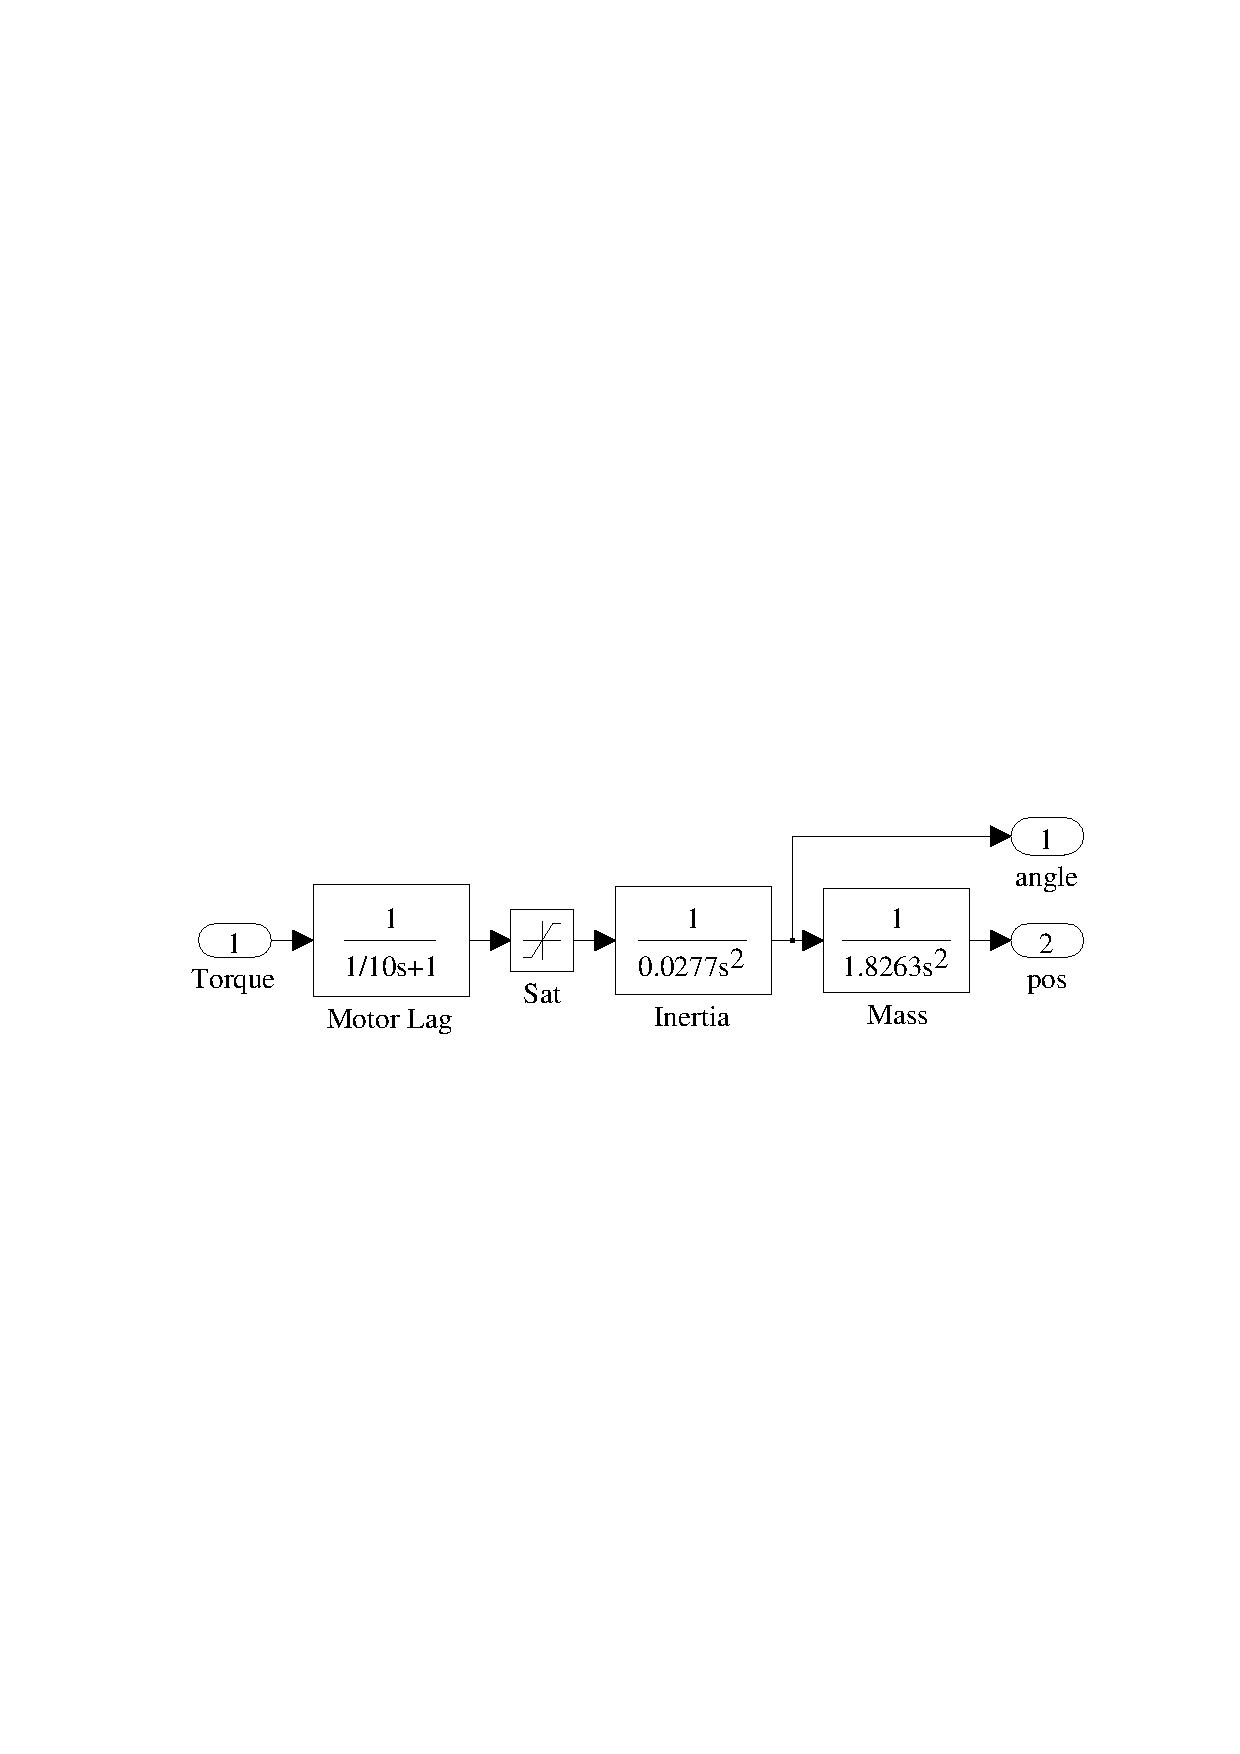
\includegraphics[width=\columnwidth]{figures/quadrotor_plant.png}
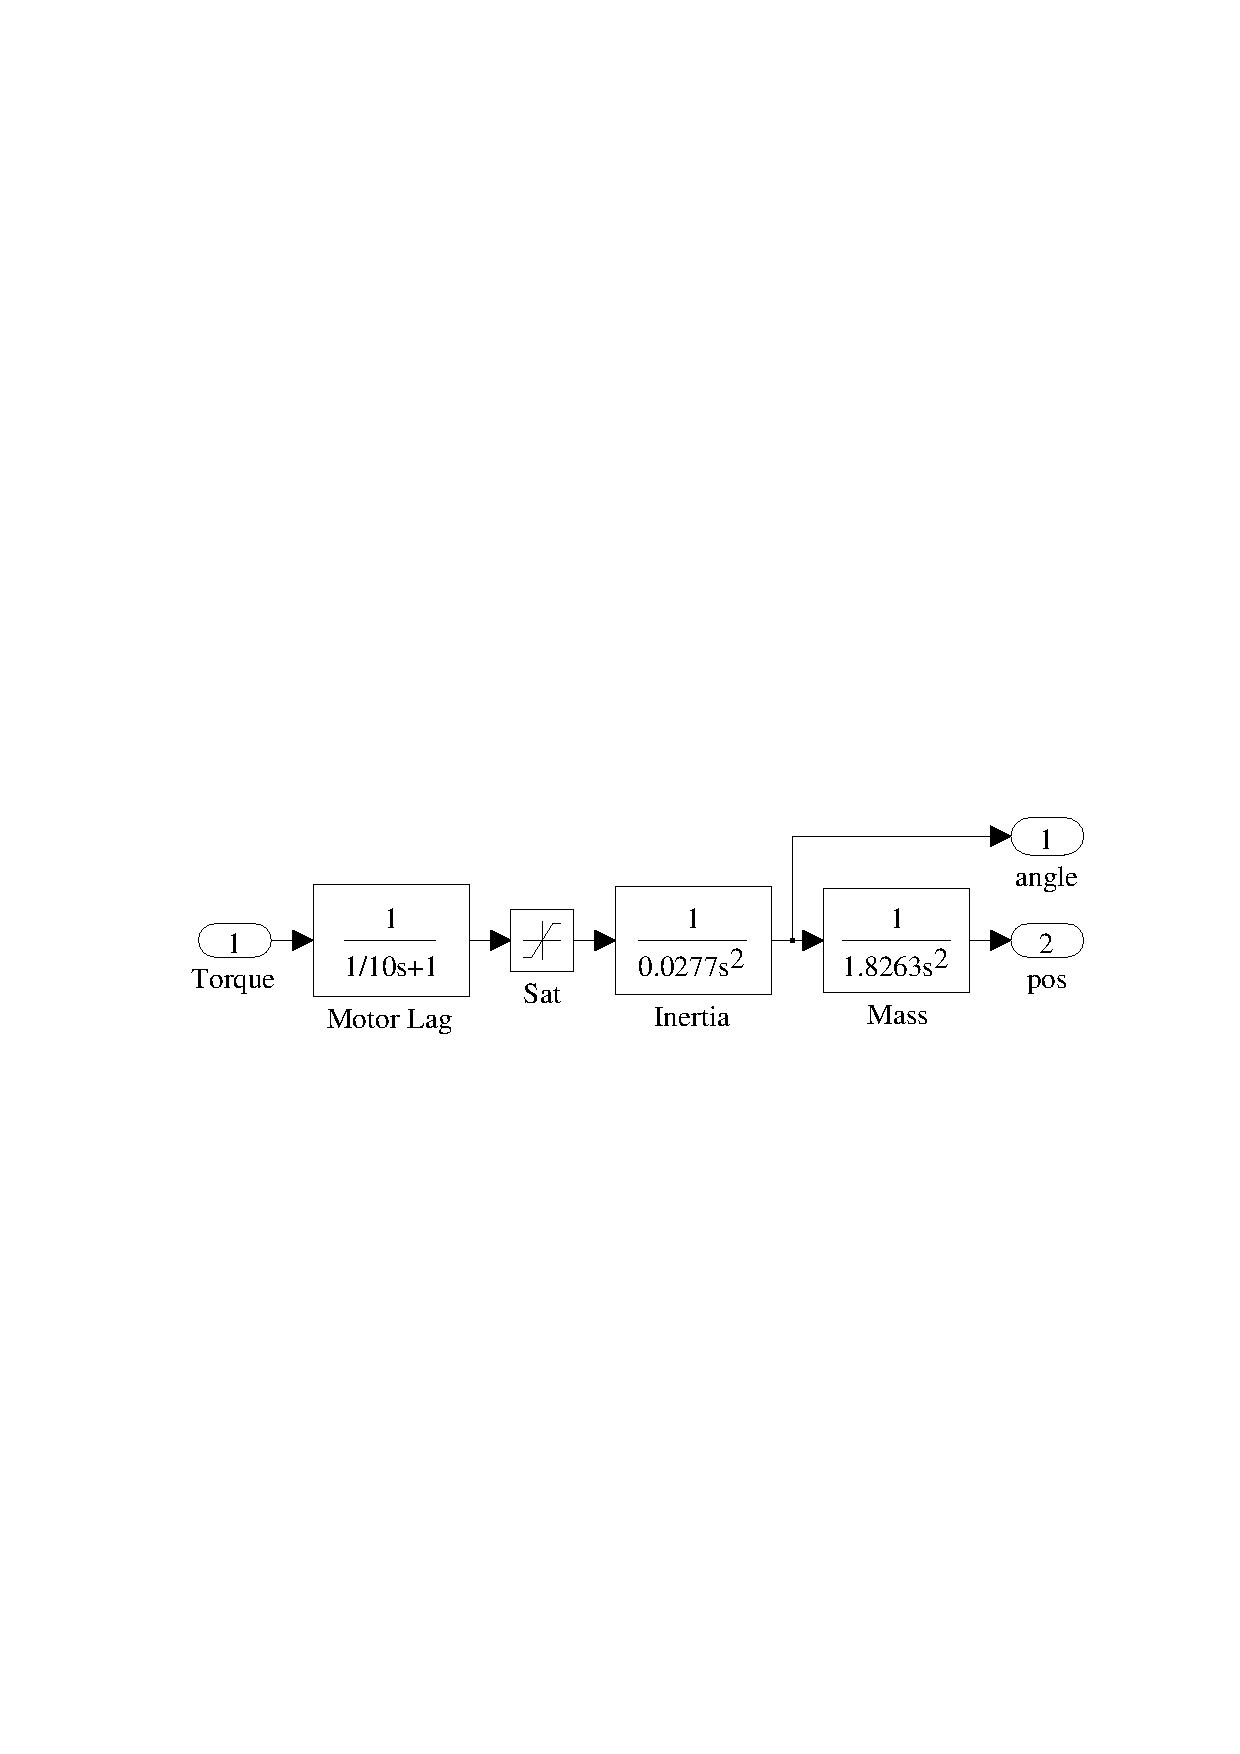
\includegraphics[width=0.5\columnwidth]{figures/quadrotor_plant.png}
    \caption{Simplified quadrotor plant dynamics.  The rotational dynamics have
been removed to facilitate easier study of the behavior.  The full model
includes all of the dynamics.  The signals lines leading off the picture are
signal taps used for online stability analysis.}
    \label{fig:qr_plant}
\end{figure}

\section{Design Example}

%\begin{wrapfigure}{r}{3in}
\begin{figure}
   \centering
%   \includegraphics[width=0.9\columnwidth]{figures/vdiagram.png}
   \includegraphics[width=4in]{figures/vdiagram.png}
   \caption{Conceptual development flow supported by the tool chain.}
   \label{fig:vdiagram}
\end{figure}
%\end{wrapfigure}

Our design example controls a continuous-time system whose model represents a simplified 
version of a quadrotor UAV.  Fig. \ref{fig:quadrotor} depicts the basic
component architecture for the control design.  Our example excludes the
nonlinear rotational dynamics of the actual quadrotor for simplicity, but
retains the difficult stability characteristics. Fig. \ref{fig:qr_plant} shows
a Simulink model containing the simplified dynamics. For the fully detailed
quadrotor model and a complete discussion of the control design philosophy, see
\cite{quad:passcontrol}. The example model controls a stack of four
integrators (and motor lag) using two nested PD control loops.
%, as shown in the
%Simulink diagram shown in Fig. \ref{fig:qr_mdl}.  
The Plant block contains the integrator models representing the vehicle dynamics. The two control loops (inner and outer, as shown in Fig. \ref{fig:qr_mdl}) are
implemented on separate processors, and the execution of the components is
controlled by a simple time-triggered virtual machine that releases tasks and
messages at pre-calculated time instants.  We refer to this example as the Quad Integrator.

% Control design centers around the continuous-time abstraction of passive control \cite{quad:passcontrol}.  
% Passivity provides a robust version of continuous-time dynamic stability which is insensitive to 
% quantization effects \cite{pass:fettweis86} and network delays \cite{ncs:chopra}\cite{ncs:wireless} 
% in digital control implementations.  The passivity conditions help relax constraints on required 
% component sample rates, increasing the system's tolerance to jitter and other timing variations. 
% 
% Simulated stability analysis yields period parameters for the control components. For 
% our discussion the exact nature of these parameters is not important, rather that they represent 
% the same behaviors for all of the integrated tools.  Passive design provides a guarantee of stable 
% operation around a nominal sampling rate, as the system will tolerate a small number of lost or 
% delayed data samples.




% Behavior of the deployed components depends on execution timing of the functions
% on the platform, the calculated schedule, and coordination between distributed
% tasks. The calculated execution schedule can be used to simulate the control
% design with additional delays to assess the impact of the platform on
% performance.  Fig. \ref{fig:delays} shows simulated effects of additional delays
% in the control data paths.  The top of the figure is the direct synchronous
% digital implementation of the control system.  The two successive plots show the
% effects of adding first one and then two extra delay elements in each control
% path.  The reference input frequency and amplitudes were chosen to lie on the
% edge of the stable operating point of the design.  This is not meant to be an
% exhaustive verification of the control design, rather an illustration of the
% gradual oscillation and overshoot degradation that occurs as delays increase.  
% 
% \begin{figure}
% \centering
% \includegraphics[width=0.9\columnwidth]{figures/delays.png}
%     \caption{Effects of increasing delays in the synchronous scheduling of the
% control nodes.}
%     \label{fig:delays}
% \end{figure}


\section{Vision}

%In this work, we envision a sophisticated, end-to-end toolchain that supports not only construction but 
%also the verification of the engineering artifacts (including software) for high-confidence applications. 
%The development flow provided by the toolchain follow a variation of the classical V-model (with 
%software and hardware development on the two branches), with some refinements added at the various 
%stages. Fig. \ref{fig:vdiagram} illustrates this development flow.

Our approach for creating high-confidence designs varies somewhat from the 
traditional V-diagram development model (see Fig. \ref{fig:vdiagram}).  In the
traditional model we move down the V, refining designs as we proceed, with the
level of integration increasing as the project progresses.  We recognize that
system integration is often the most costly and difficult part of development.
Lessons learned during integration frequently occur too late to benefit project
decision-making.  We aim to automate much of the integration work, and therefore
shorten design cycles.  Beyond that, we want to enable feedback of models and
analysis results from later design stages back to earlier design cycles (via
the dashed lines in the diagram) to facilitate rapid rework if necessary.  The
goal is that the overall project can rapidly move towards a correct implementation.

%\begin{wrapfigure}{l}{3.2in}
\begin{figure}
\centering
%\includegraphics[width=0.9\columnwidth]{figures/designflow.png}
\includegraphics[width=4.2in]{figures/designflow.png}
    \caption{Flow of design models between design phases. }
    \label{fig:designflow}
\end{figure}
%\end{wrapfigure}

Consider the general class of control system designs for use in a flight control system.  Sensors, 
actuators, and data networks are designed redundantly to mitigate faults.  The underlying platform 
implements a variant of the time-triggered architecture (TTA)~\cite{timed:tta}, which provides 
precise timing and reliability guarantees.  Safety-critical tasks and messages execute according to 
strict precomputed schedules to ensure synchronization between replicated components and provide fault 
mitigation and management.  Software implementations of the control functions must pass strict 
certification requirements which impose constraints on the software as well as on the development 
process.  

Figure \ref{fig:designflow} depicts a design flow that includes a user-facing modeling language 
for design and an abstract intermediate language for supporting interpreter development and
maintenance.  During design, a software modeler imports an existing Simulink control design into 
the Generic Modeling Environment (GME) \cite{mic:gme}, configured to edit ESMoL models.  The modeler
then uses the dataflow models imported from Simulink to specify the functions of software components
that will implement the controllers.  These components are extended with interfaces defining their 
input and output message structures.  The components are instantiated into multi-aspect models where 
logical dependencies, hardware deployment, and timing models can be specified for the software architecture.
The completed model is transformed (via the Stage 1 transformation) into a model in the 
ESMoL\_Abstract language, where all implied relationships and structural model inferences have been resolved.  
Model interpreters for calculating time-triggered schedules, creating platform-specific simulations, and
generating deployable code are integrating using the Stage 2 transformation.


%A modeling language to support this development flow must have several desired properties:  (1) the 
%ability to capture the relevant aspects of the system architecture and hardware, (2) ability to 
%``understand'' (and import) functional models from existing design tools, (3) support for 
%componentization of functional models, and (4) ability to model the deployment of the software 
%architecture onto the hardware architecture. The ability to import existing models from functional 
%modeling tools is not a deeply justified requirement, it is merely pragmatic.  A simple sample design will introduce key points of our model-based 
%development flow and illustrate language concepts.  

%Our language design was influenced by two factors: (1) the MoC implemented by the platform and (2) the 
%need for integration with legacy modeling and embedded systems tools. We have chosen Simulink/Stateflow 
%as the supported ``legacy'' tool. As our chosen MoC relies on periodically scheduled time-triggered 
%components, it was natural to use this concept as the basis for our modeling language and interpret the 
%imported Simulink blocks as the implementation of these components. To clarify the use of this 
%functionality, we import a Simulink design and select functional subsets which execute in discrete time, 
%and then assign them to software components using a modeling language that has compatible 
%(time-triggered) semantics. Communication links (signals) between Simulink blocks are mapped onto TTA 
%messages passed between the tasks. The resulting language provides a componentized view of Simulink 
%models that are scheduled periodically (with a fixed rate) and communicate using scheduled, 
%time-triggered messages.  Extensions to heterogeneous MoC-s is an active area of research.

\subsection{Requirements Analysis (RA)}

%Our running example will model a data network implementing a single sensor/actuator loop with a 
%distributed implementation.  The sensors and actuators in the example are doubly-redundant, while the 
%data network is triply-redundant.  The common nomenclature for this type of design is TMR (triple modular 
%redundancy).  Unlike true safety-critical designs, we will deploy the same functions on all replicas 
%rather than requiring multiple versions as is often done in practice~\cite{std:DO178B}.  The sensors and 
%actuators close a single physical feedback loop.  Specifying the physical system and particulars of the 
%control functions are beyond the scope of this example as our focus is on modeling.

This example has an informal set of requirements, though our modeling language currently supports the 
formalization of timing constraints between sensor and actuator tasks.  Formal requirements modeling 
offers great promise, but in ESMoL requirements modeling is still in conceptual stages.  We discuss latency modeling structures in a later example.

% A simple 
%sensor/actuator latency modeling example appears in a later section covering preliminary features for the 
%language.

Informally, we require stability of the closed-loop system over the full range
of possible inputs.  Performance should allow reasonable tracking of a reference
trajectory within the physical limits of the vehicle.

\subsection{Functional Design (FD)}

%\begin{figure}
%	\centering
%   \includegraphics[width=\columnwidth]{figures/sl_design.png}
%   \caption{Simulink design of a basic signal conditioner and controller.}
%   \label{fig:sl_design}
%\end{figure}

In ESMoL, functional specifications for components can appear in the form of Simulink/Stateflow models or 
as existing C code snippets.  ESMoL does not support the full semantics of Simulink. In ESMoL the execution 
of Simulink data flow blocks is restricted to periodic discrete time, consistent with the underlying 
time-triggered platform.  This also restricts the type and configuration of blocks that may be used in a 
design.  Continuous integrator blocks and sample time settings do not have meaning in ESMoL.  C code 
snippets are allowed in ESMoL as well.  C code definitions are limited to synchronous, bounded response 
time function calls which will execute in a periodic task.

% \begin{figure}
% 	\centering
%    \includegraphics[width=\columnwidth]{figures/esmol_design.png}
%    \caption{ESMoL-imported functional models of the Simulink design.}
%    \label{fig:esmol_design}
% \end{figure}

Fig. \ref{fig:qr_mdl} shows a simple top-level Simulink design for the quadrotor model.
%TODO: Get the right figure for this. 
% along with the imported ESMoL model (Fig. \ref{fig:esmol_design}).  
The imported ESMoL model is a structural replica of the 
original Simulink model, only endowed with a richer software design environment and tool-provided APIs for 
navigating and manipulating the model structure in code.  A model import utility provides the illustrated 
function.

\subsection{Component Design (CD)}

\begin{figure}
\centering
%\includegraphics[width=0.9\columnwidth]{figures/quadrotor_types.png}
\includegraphics[width=0.75\columnwidth]{figures/quadrotor_types.png}
    \caption{The component type model specifies message types and fields, as well as component types.  Component types specify the mapping of Simulink functional designs to the fields in the messages that will carry the data.  These components and messages are instantiated in the architecture and deployment models.}
    \label{fig:qr_types}
\end{figure}

In the component design phase (CD) we specify interfaces for the functions which will run in the 
distributed controller network.  A component specification contains a reference to a Simulink subsystem,
as well as references to message structure objects.  The message structure objects will represent message
types, and each reference from a component definition represents an interface through which that message
is sent or received.  Internally, the direction of the connection from the message reference to the ports
on the Simulink object determine whether the port sends or receives.  We do not allow multi-directional
message transfers on the same interface.  When the component is instantiated in other parts of the design
(e.g., in the logical architecture diagram described below) the message references specified here will 
appear as ports on the instance.  Connections to and from those ports represent the transfer of that
data message into or out of the component.

Fig. \ref{fig:qr_types} shows an example of the component interface definition 
language.  Message fields and their sizes are specified here, as well as
component implementations and interfaces.  These specifications are types in
an ESMoL model, and they are instantiated in the architecture and 
deployment models.  The quad integrator model has four
different component types (each instantiated once) and six message types
(instantiated as the ports objects appearing on the component instances later
in the design).  The breakout in the figure shows the internals of the DataHandler component
specification.  The block in the center is a reference to the Simulink block that specifies
its functional behavior.  The blocks on the outer edges are references to messages defined at
the top level of the system types model.  The connections between the message ports and the
Simulink reference block ports describe the direction and details of data flow between the 
implemented message structures and the specified functional block.

In the component types sublanguage a component may be implemented by either a Simulink Subsystem or a 
C function.  They are compatible at this level, because here their model elements represent the code that 
will finally implement the functions.  They are assumed to execute synchronously.  These units are 
modeled as blocks with ports, where the ports represent parameters passed into and out of C function calls.

\begin{figure}
\centering
%\includegraphics[width=0.9\columnwidth]{figures/quadrotor_log_arch.png}
\includegraphics[width=0.75\columnwidth]{figures/quadrotor_log_arch.png}
    \caption{The logical architecture aspect specifies data
dependencies between software component instances. The ports on the blocks
represent data messaging interfaces into and out of the component.}
    \label{fig:qr_log_arch}
\end{figure}

\subsection{Logical Software Architecture (SwA)}


%\begin{figure}
%	\centering
%   \includegraphics[width=0.9\columnwidth]{figures/tmr_arch.png}
%   \caption{The logical architecture diagram defines data dependencies, and gives finer control over 
%instantiation of functional units.}
%   \label{fig:tmr_arch}
%\end{figure}

\begin{figure}
\centering
%\includegraphics[width=\columnwidth]{figures/qr_tmr.png}
\includegraphics[width=0.75\columnwidth]{figures/qr_tmr.png}
    \caption{Triply-redundant version of the quadrotor logical architecture to illustrate instantiation in
ESMoL design models.  Each of the quadrotor design components is instantiated multiple times in this model.}
    \label{fig:qr_tmr}
\end{figure}

Fig. \ref{fig:qr_log_arch} portrays logical data dependencies between
software component instances, independent of their distribution over different
processors.  The software architecture model describes the logical 
interconnection of component instances.  
Semantics for SwA Connections are those of task-local synchronous function 
invocations as well as message transfers between tasks using time-triggered 
communication.  The logical architecture, deployment, and timing/execution
models represent different design aspects for the same set of component 
instances.  GME allows us to define the language in such a way that these three
model aspects are simply different views of the same set of model elements.

Creation of a (GME) reference object to one of the component types corresponds to instantiation.
The architecture design model aspects (logical architecture, deployment, and timing) allow us to
perform software design with components whose functions are specified by Simulink dataflow diagrams.
Fig. \ref{fig:qr_tmr} illustrates this idea.  Using the same controller components along with a few new
components to implement voting logic, we have specified the logical architecture for a triply-redundant
version of the quadrotor model.  This assumes that the hardware support is all available, and could be
specified in the hardware and deployment models -- this particular model diagram is only shown to 
illustrate the instantiation mechanism.

\subsection{Hardware Architecture (HwA)}

\begin{figure}
  \centering
%  \includegraphics[width=\columnwidth]{figures/quadrotor_hardware.png}
  \includegraphics[width=0.75\columnwidth]{figures/quadrotor_hardware.png}
  \caption{Overall hardware layout for the quadrotor example.}
  \label{fig:qr_hardware}
\end{figure}

Hardware configurations are explicitly modeled in the platform language.  Platforms are defined 
hierarchically as hardware units with ports for interconnections. Primitive components include processing 
nodes and communication buses.  Behavioral semantics for these networks come from the underlying 
time-triggered architecture.  The time-triggered platform provides services such as deterministic 
execution of replicated components and timed message-passing.  Model attributes for hardware also 
capture timing resolution, overhead parameters for data transfers, and task context switching times.

Fig. \ref{fig:qr_hardware} illustrates an example of a platform model.  The quadrotor architecture
is deployed to a small embedded processor assembly manufactured by Gumstix, Inc.
The position control is handled by an Intel PXA ARM processor (the Gumstix 
board), and attitude control and vehicle I/O are handled by an Atmel 
Atmega128 AVR processor (the Robostix board).  The I/O occurs over serial 
connections to the sensors and motor actuators.  The serial devices reside on
the processor, and are modeled in the diagram as objects connecting the 
input and output ports on the processor to the object representing the plant
dynamics.  The two processors communicate via a synchronous I2C bus which runs
a software emulated time-triggered protocol.

% \begin{figure}
% 	\centering
%    \includegraphics[width=0.9\columnwidth]{figures/platformex.png}
%    \caption{Detail of hardware model for controller units.}
%    \label{fig:platformex}
% \end{figure}
% 
% Figs. \ref{fig:tmr_hardware} and \ref{fig:platformex} show model details for redundant hardware elements.  Each controller unit is a private network with two nodes and three independent data buses.
% Sensor voting and flight control instances are deployed to the controller unit networks.



\subsection{Deployment Models (SY, DPL)}

%\begin{figure}
%	\centering
%   \includegraphics[width=0.9\columnwidth]{figures/tmr_deploy.png}
%   \caption{Deployment model: task assignment to nodes and details of task definition.}
%   \label{fig:tmr_deploy}
%\end{figure}

\begin{figure}
\centering
\includegraphics[width=0.75\columnwidth]{figures/quadrotor_hw_mapping.png}
    \caption{The platform deployment aspect specifies the hardware
components that will support the transfer of data to and from each processing
node, the software components that will send and receive the data, and the
message instances in which the data will be carried.  Dashed arrows represent
assignment of components to their respective processors, and solid lines
represent assignment of message instances (component ports) to communication
channels (port objects) on the processor.}
    \label{fig:qr_hw_mapping}
\end{figure}

Fig. \ref{fig:qr_hw_mapping} shows the deployment model -- the mapping
of software components to processing nodes, and data messages to communication
ports.  Two of the four components are mapped to each of the two processors.  RS
(Robostix) is an 8 bit ATMega128 CPU, and GS (Gumstix) is an Intel PXA ARM-based CPU.



The deployment aspect captures the assignment of component instances as periodic tasks running 
on a particular processor.  In ESMoL a task executes on a processing node at a single periodic rate.  All 
components within the task execute synchronously.  Data sent between tasks takes the form of messages in 
the model.  Whether delivered locally (same processing node) or remotely, all inter-task messages are 
pre-scheduled for delivery.  ESMoL uses logical execution time semantics found in time-triggered 
languages such as Giotto~\cite{timed:giotto} -- message delivery is scheduled after the deadline of 
the sending task, but before the release of the receiving tasks.  In the TT model message receivers 
assume that required data is already available at task release time.  Tasks never block, but execute with 
whatever data is available each period.

Deployment concepts -- tasks running on processing nodes and messages sent over data buses -- are modeled 
as shown in Fig. \ref{fig:qr_hw_mapping}.  The dashed connection from a component to a node reference 
represents an assignment of that component to run as a task on the node.  The port connections represent
the hardware channel through which that particular message will travel.  Remote message dependencies 
are assigned to bus channels on the node.  Local data dependencies are not specified here, as they are
represented in the logical architecture.  IChan and OChan objects on the node can also be connected to 
message objects on a component.  These connections represent the flow of data from the physical 
environment through sensors (IChan objects) or the flow of data back to the environment through actuators
(OChan objects).  Model interpreters use deployment models to 
generate platform-specific task wrapping and communication code as well as analysis artifacts.

\subsection{Timing Models}

\begin{figure}
\centering
%\includegraphics[width=\columnwidth]{figures/quadrotor_timing.png}
\includegraphics[width=0.8\columnwidth]{figures/quadrotor_timing.png}
   \caption{The timing/execution model indicates which components and
messages will be scheduled independently.  In the case of
processor-local data transfers transfer time is neglected, as reads and
writes occur in locally shared memory.  The time order of the message writer 
and readers are enforced by the static schedule. The locality of a message transfer is
specified in the architecture and deployment models.  GME provides a separate
window (not shown) for editing object parameters and attributes.}
   \label{fig:qr_timing}
\end{figure}

Fig. \ref{fig:qr_timing} shows a timing and execution model for the quad integrator, which allows 
the designer to attach timing parameter
blocks to components and messages.  For the time-triggered case the configuration 
parameters include execution period and worst-case execution time.  The quad integrator
model runs all of the blocks at a frequency of 50Hz.  The execution model also indicates 
which components and messages will be scheduled independently, and which will be
grouped into a single task or message object.  Our example model assigns each component to its own task.  For calculated static schedules start times are also 
stored in the timing objects after the analysis has been performed.

\section{Key Techniques and Technologies}
\label{sect:esmolkey}

\begin{figure}
	\centering
%	\includegraphics[width=\columnwidth]{figures/platform.png}
	\includegraphics[width=0.8\columnwidth]{figures/platform.png}
	\caption{Platforms. This metamodel describes a simple language for modeling the topology of a time-triggered processing network.  A sample platform model is included.}
	\label{fig:platform}
\end{figure}

The models in the example and the metamodels described below were created using the ISIS Generic 
Modeling Environment tool (GME)~\cite{mic:gme}.  GME allows language designers to create 
stereotyped UML-style class diagrams defining metamodels.  The metamodels are instantiated into a 
custom domain-specific graphical language, and metamodel class stereotypes and attributes determine how the elements are 
presented and used by modelers. 

The Model-Integrated Computing approach\cite{mic:overview} builds up DSMLs by creating specific
sublanguages to capture concepts and relationships for different facets of the
design domain, and then integrating those sublanguages into a common modeling
language by precisely specifying the structural relationships between those 
sublanguages.



The Simulink and Stateflow sublanguages of our modeling environment are described elsewhere, though the 
ESMoL language changes many of the other design concepts from previously developed languages described by 
Neema~\cite{mic:ecsldp}.

Another key technology used in the ESMoL tool suite is the GReAT model transformation language (and its
associated code generation tools)\cite{mic:great}.  ESMoL contains a pair of platform-independent code
generators for Simulink and Stateflow models.  The transformations take Simulink and Stateflow blocks, and
create equivalent models in another language (SFC) that corresponds to an abstract syntax graph for 
fragments of C code.  Functional code generation proceeds by simply traversing and printing the SFC 
models. Other generators create code implementing the platform-specific code to wrap functions as tasks, 
define communication messages structures, and configure a time-triggered virtual machine to execute the
generated code.  These generators as well as generators for platform-resimulation models are described
elsewhere (see Porter et al \cite{modeling:esmol}, Thibodeaux \cite{timed:frodo}, and Hemingway et al
\cite{modeling:truetime} for details).

High-confidence systems require platforms providing services and guarantees for properties such as fault 
containment, temporal firewalls, and partitioning.  System developers should not re-implement such 
critical services from scratch~\cite{modeling:platform}.  The platform also defines a 
model of computation (MoC) \cite{sem:taggedsig}. A MoC governs how the concurrent objects of an 
application interact (i.e. synchronization and communication).  Our chosen MoC is the time-triggered
architecture (TTA)\cite{timed:tta}.  The time-triggered architecture provides deterministic synchronous
execution in order to ensure the consistent behaviors of distributed replicas of controller components.  

% The described approach is part of the ESMoL modeling language and software design 
% suite\cite{modeling:aces08}.  ESMoL is a research experiment in the implementation of modeling 
% tools to support compositional analysis and design frameworks.  In our design flow a modeler 
% imports Simulink/Stateflow models \cite{tools:mathworks} into the ESMoL language, adds architecture 
% elements, platform design, and deployment concepts, then performs automated analysis and synthesizes 
% code for execution on a time-triggered platform.  We aim to support iterative
% development, as analysis data can flow back to earlier stages for re-design or
% re-evaluation.  The language and tools also include preliminary support for
% requirements modeling, by allowing specification of maximal latency 
% bounds between computational tasks in the design.

% Table
%\ref{tab:consistencyTools} gives an overview of our toolchain design goals and
%philosophy, considering details from three different semantic models.



%\begin{table*}
%	\centering
%		\begin{tabular}[width=0.75\columnwidth]{@{\extracolsep{\fill}} |
%p{1.7cm} | p{4.6cm} | p{4.6cm} | }
%		\hline
%		\multicolumn{3}{|c|}{Behavioral Model Interactions} \\
%		\hline
%		. & Execution Order Constraints & Timing Constraints \\ \hline \hline
%		Stability (Comp) & Passive controllers run synchronously at a fixed rate determined by control analysis and simulation. & Control functions execute in bounded time, measured for the given platform. Nominal sample rates are passive and stable. \\ \hline
%		Stability (Intr) & Passive control design decreases the effects of delays from scheduling and platform timing jitter. Maximum acceptable sample delay is one possible abstraction for these effects. & Timing guarantees are not yet considered in our passive control design framework. \\ \hline
%		\hline
%		Scheduling (Comp) & We use a synchronous execution model to precompute component invocation order within tasks to eliminate local data hazards. & Each task has a known, bounded execution time (WCET/Deadline parameters are in the model).  \\ \hline
%		Scheduling (Intr) & Message and task dependencies are translated to linear constraints, along with constraints to model resource utilization. & Scheduling achieves the desired sample rate and enforces latency bounds between tasks.  A proposed delay abstraction could represent schedule slack, and latency could be used to budget slack. \\ \hline
% \hline
%		Execution Environment (Comp) & Statically precomputed task
%release times are used to configure the generated tasks, and the VM enforces
%start times. & We assume bounded-time task execution.  VM tasks can not be
%preempted, and so execute as quickly as possible to meet their deadline (WCET in
%this case). \\ \hline
%		Execution Environment (Intr) & Clocks on separate nodes are
%synchronized to support synchronous execution.  Frame sync (null) messages are
%sent at the start of the common hyperperiod to keep nodes executing together.  &
%Time-triggered schedules prevent collisions, so messages transfer
%deterministically. Measured transfer overhead is captured in the platform
%design, and used in scheduling calculations. \\ \hline
%		\end{tabular}
%	\caption{Summary discussion of the behavioral consistency goals from the
%point of view of each design stage of our tools so far.  The table covers
%relationships between three different semantic models: dynamic stability,
%schedulability, and deadlock freedom. The (Comp) notation refers to local
%(component/task) level concerns, and (Intr) refers to design concerns at the
%level of interactions between components, consistent with our platform
%abstraction.  The ESMoL language constructs should embody the correct
%resolution of these design issues, and maintain the assumptions through all
%stages of design and execution.}
%	\label{tab:consistencyTools}
%\end{table*}
%

\section{ESMoL Language Details}

\begin{figure}
	\centering
	%\includegraphics[width=\columnwidth]{figures/arch_lang.png}
	\includegraphics[width=0.85\columnwidth]{figures/arch_lang.png}
	\caption{System Types Metamodel. Architecture models use instances of Simulink subsystems or 
C code functions to specify the functionality of software components, adding attributes for real-time execution. The Input and Output port
classes are typed according to the implementation class to which they belong. The connections between the block reference and the MsgPort objects describe the details required to marshal and demarshal messages for use by the specified function.}
	\label{fig:arch}
\end{figure}

\begin{figure}
	\centering
	%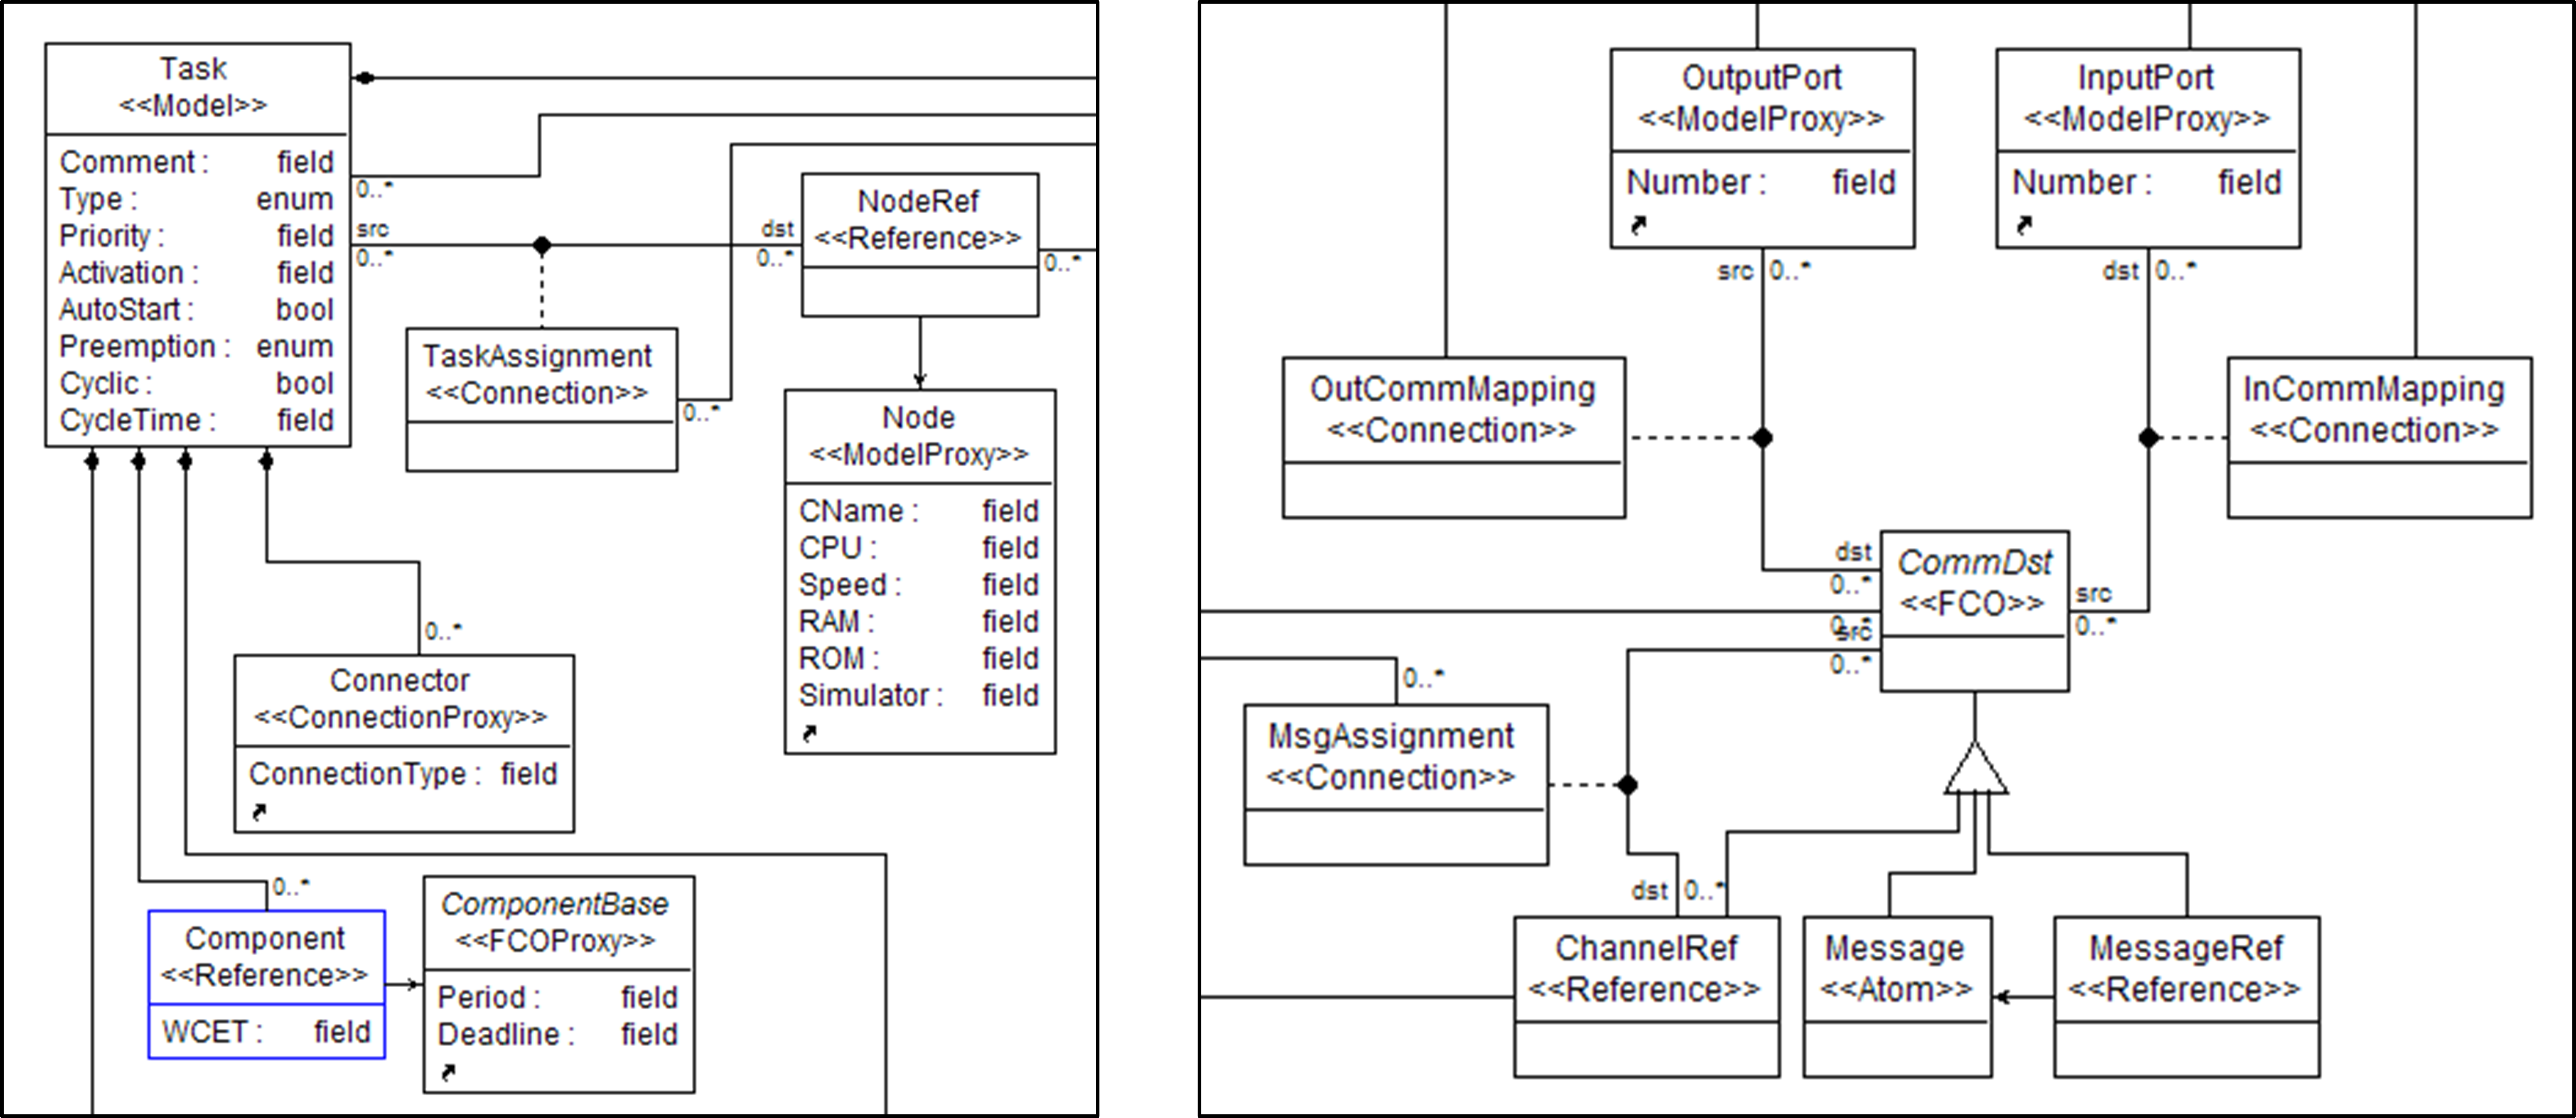
\includegraphics[width=\columnwidth]{figures/depnew.png}
	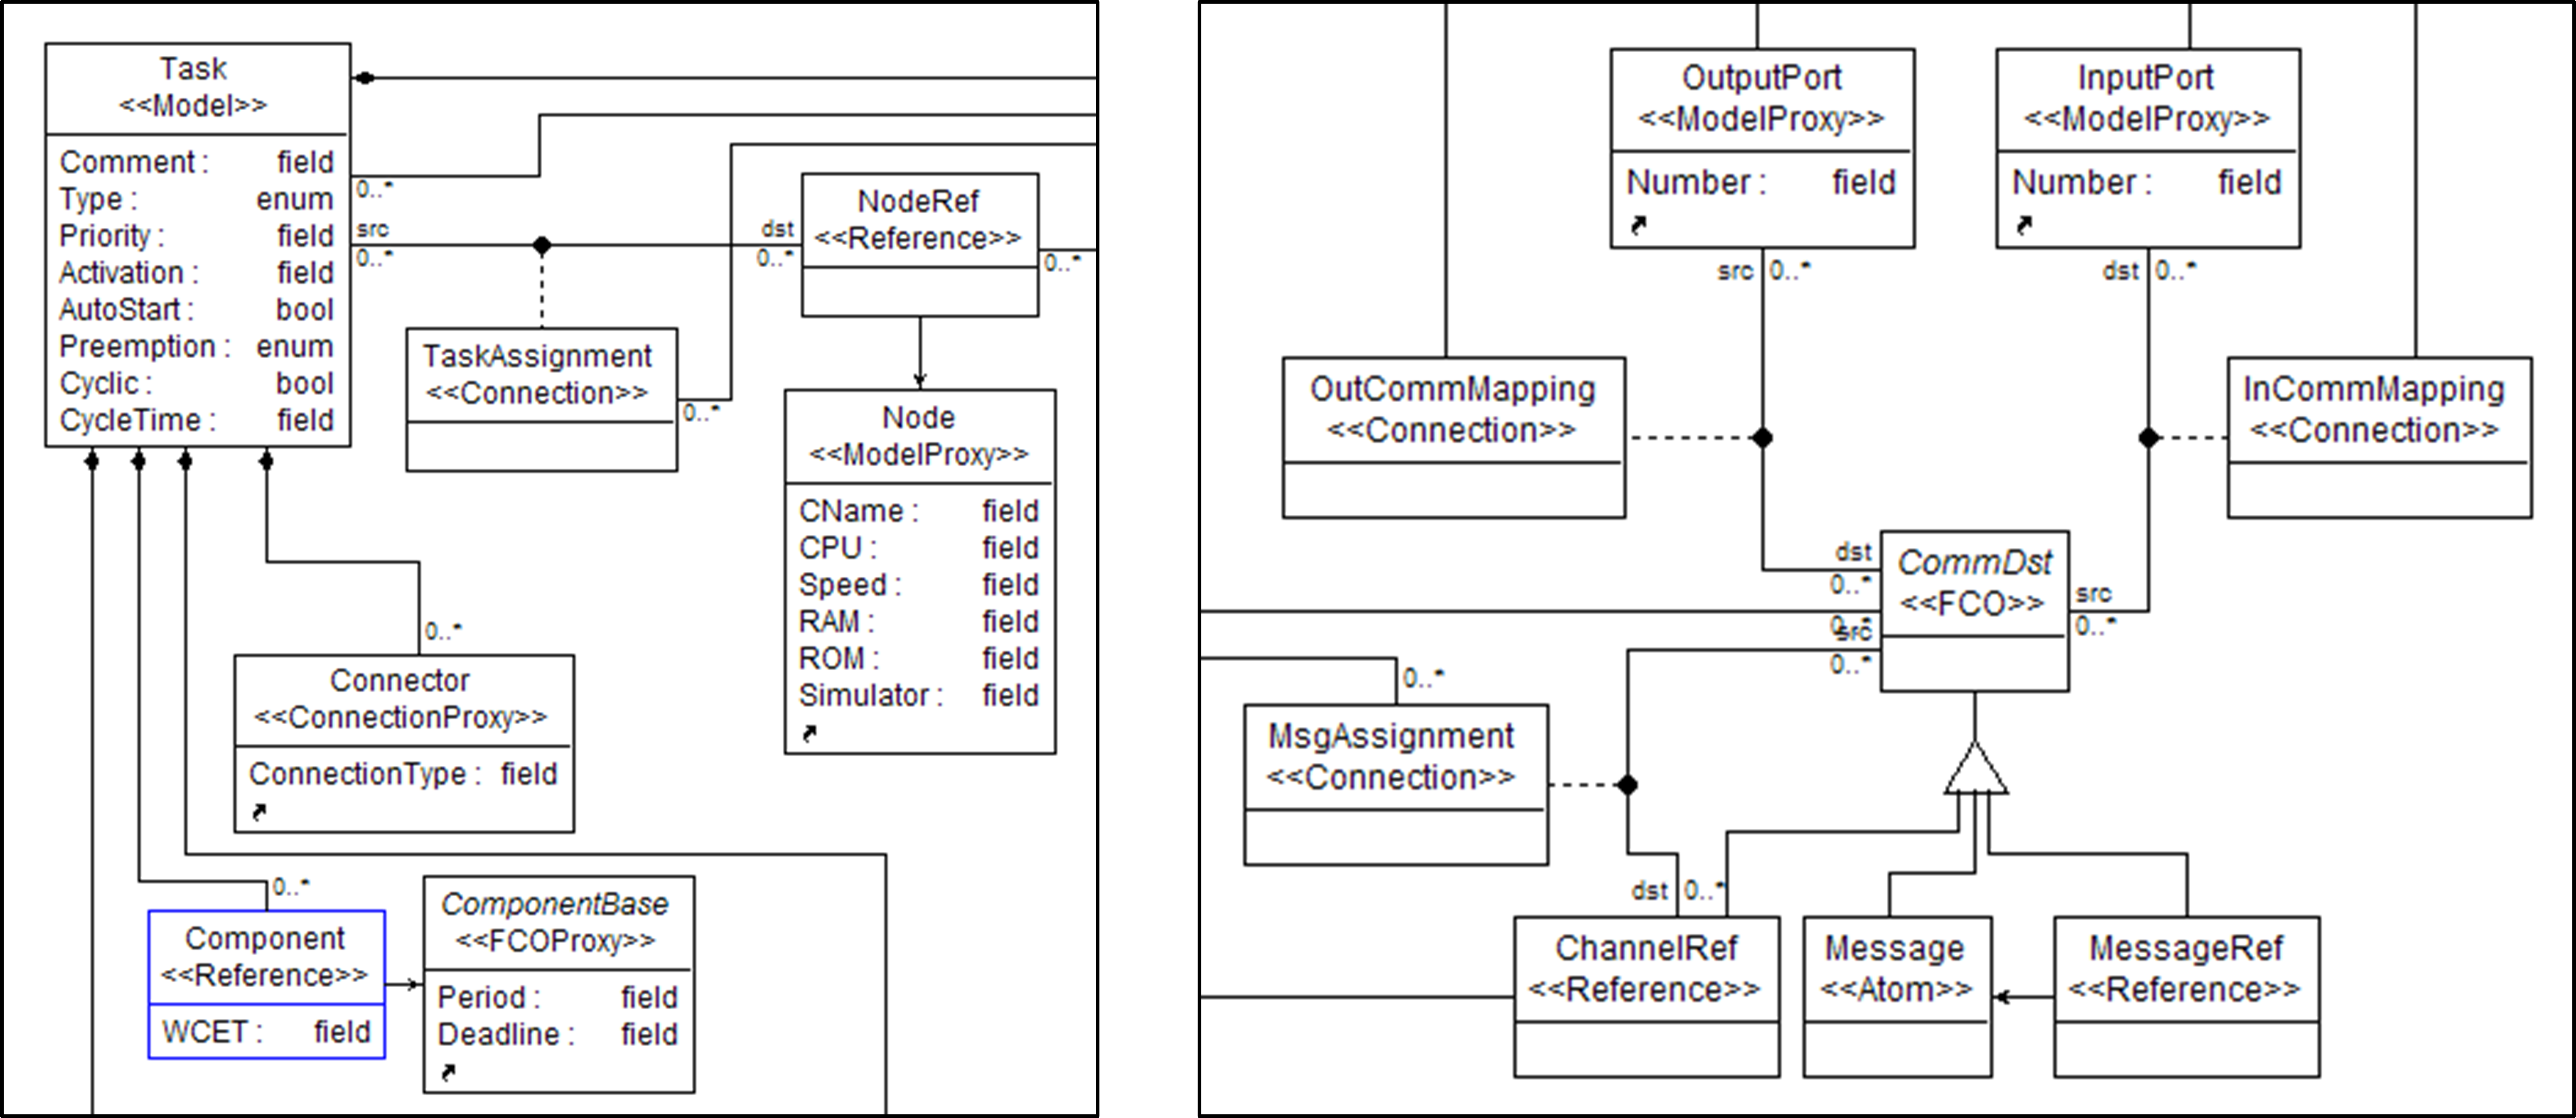
\includegraphics[width=0.85\columnwidth]{figures/depnew.png}
	\caption{Details from Deployment sublanguage.}
	\label{fig:depnew}
\end{figure}

\begin{figure}
	\centering
	%\includegraphics[width=\columnwidth]{figures/timing.png}
	\includegraphics[width=0.85\columnwidth]{figures/timing.png}
	\caption{Details from Timing sublanguage.}
	\label{fig:timing_lang}
\end{figure}

 The GME metamodeling syntax may not be entirely familiar to the reader, 
but it is well-documented in Karsai et al~\cite{mic:gme}. Class concepts such as inheritance can be 
read analogously to UML.  Class aggregation represents containment in the modeling environment, though 
an aggregate element can be flagged as a port object.  In the modeling environment a port object will 
also be visible at the next higher level in the model hierarchy, and available for connections.  
One unique notation in MetaGME (the GME modeling language for creating modeling languages) is the dot
used for relating an association class to its endpoint connection classes.  For example, the dot 
between the Connectable class and the Wire class (Fig. \ref{fig:platform}) represents a line-style 
connection in the modeling environment.

A simple platform definition language (Fig. \ref{fig:platform}) contains relationships and attributes 
describing time-triggered networks.  The models contain network topology and parameters to describe 
behavioral quantities like data rates and bus transfer setup times.

Fig. \ref{fig:arch} portrays the System Types sublanguage.  Components of different types (here 
Simulink block references or C code blocks) specify the component functions.  Message references 
define interfaces on the components, and ports on those message represent message data fields.  
Directed connections between the functional block and the message field ports represent marshaling
and demarshaling of message data as it is consumed and produced by the specified component functions.

The Fig. \ref{fig:depnew}  metamodel illustrates the classes and relationships for both the logical
architecture connections and the deployment mapping.  GME metamodels have a separate visualization 
aspect that allows us to define aspects in ESMoL and indicate which classes and connections should be
visible in each aspect.  ComponentRef objects are instances in ESMoL, and are visible in both aspects.
In the logical architecture aspect, Dependency connectors define message transfers between component 
instance ports.  The ports represent interfaces for each component instance.  For the deployment aspect
we add the NodeRef object (node references) and connectors (ComponentAssignment and CommMapping) to identify
the mapping of tasks and messages to the platform model.

The timing sublanguage (Fig. \ref{fig:timing_lang}) allows the designer to specify component execution
constraints.  Individual components can be annotated with timing objects that indicate 
whether they should be executed strictly (i.e., via statically scheduled time-triggered means), or as
periodic real-time or sporadic tasks.  Components can also be grouped into a task.  Messages are similarly
annotated.  The annotation objects contain parameters such as period and worst-case execution time that
must be given by the designer.  Automated scheduling analysis fills in the schedule fields.

\section{Interpreter Development Architecture}
\label{sect:twostage}

In the model integrated computing approach, domain specific modeling languages represent 
different aspects of the design, with the aim  of consistently integrating different concepts and details for those design aspects and integrated analysis tools.
Our approach can be considered as an implementation of the tool integration ideas 
in \cite{modeling:hybrid_abs}, but with variations of the details included in the design language.  
Specifically we propose the following main ideas:

\begin{enumerate}

\item A front end graphical modeling language which integrates into existing 
design workflows\cite{modeling:esmol}.  This has already been described (ESMoL).

\item A single transformation from front end models to an intermediate language explicitly 
representing a flattened semantic model, including parameters and objects to imply a precise 
behavioral semantics.  We differ from the approach in \cite{modeling:hybrid_abs} by abstracting the 
dynamic component interface behavior using passive control design 
techniques. We rely on the resulting robustness and compositionality of the passive approach 
to simplify design analysis and implementation, as our design language is
specific to distributed embedded control systems.  Note that we only have preliminary 
support for passive control design and analysis -- this is a work in progress (see \cite{ncs:mic} 
for preliminary work in this area).

\item Both the front-end and intermediate languages support platform-based design \cite{modeling:platform}, 
separating component-level concerns and interaction concerns where possible.  For detailed interaction models we use the the time-triggered 
architecture\cite{timed:tta} as a formal distributed model of computation. For
local component behavior the semantics are given by synchronous data flow. The 
tool suite supports deployment
to a time-triggered execution environment\cite{timed:frodo} in order to preservesynchronous execution semantics, preserving correctness properties that rely
on synchrony.

\item Generation of analysis models and code from the intermediate language
using simple template generation techniques\cite{sched:analysis}.

\item Representation of structural and behavioral concepts from the 
intersection of the semantic domains of integrated tools as concepts, classes,
or constraints in the front end language.

\item Round-trip incorporation of calculated analysis results into the modeling environment to 
maintain consistency as models pass between design phases.

\end{enumerate}

  Rather than designing
a user-friendly graphical modeling language and directly attaching translators
to analysis tools via model navigation APIs\cite{mic:udm}, we created a 
simpler abstract intermediate language whose
elements are similar to those of the user language. The first model
transformation (Stage1) flattens the user model into the abstract intermediate 
form, translating parameters and resolving inferences and special cases as 
needed. Generators 
for code and analysis are attached to the abstract modeling layer (in the 
Stage2 interpreter), so the 
simpler second-stage transformations are easier to maintain, and are isolated 
from changes to the user language.

Our tools enforce a single view of structural inference in the design model. We
will cover some of the transformation details to illustrate this concept.

\subsection{Stage 1 Transformation}
\label{sect:stage1}

%TODO: What is being inferred from ESMoL and represented explicitly in ESMoL_Abstract?

\begin{table*}
\centering

\begin{tabular}[width=0.5\columnwidth]{ | l | l | }
 \hline
 \textbf{Specified ESMoL Relation Sets} & \textbf{ESMoL\_Abstract Relation} \\
 \hline \hline
                                                                        & \\
 $CA_{id_N} = \{ (obj_{Node}, obj_{CompInst} ) \, |$                    & \\
 \hspace{1.7cm} $ id(obj_{Node}) = id_N \} $                            & \\
                                                                        & \\
 $AC_{id_{Ch}} = \{ (obj_{IChan}, obj_{MsgInst} ) \, |$                 & 
$ Acq = \{(obj_{MsgInst}, obj_{CompInst}, $  \\
 \hspace{1.6cm} $id(obj_{IChan}) = id_{Ch} \} $                         & 
\hspace{1.3cm} $obj_{N}, obj_{Ch}) \, |$ \\
                                                                        &  
\hspace{0.8cm} $(obj_{N}, obj_{CompInst}) \in CA_{id_N}$ \\
 $NC_{id_N} = \{ (obj_{Node}, obj_{IChan}) \, | $                       & 
\hspace{0.5cm} $ \wedge \, (obj_{Ch}, obj_{MsgInst}) \in AC_{id_{Ch}}$ \\
 \hspace{1.35cm} $id(obj_{Node}) = id_N $                                &
\hspace{0.5cm} $ \wedge \, (obj_{N}, obj_{IChan}) \in NC_{id_N}$ \\ 
 \hspace{1cm} $ \wedge \, parent(obj_{IChan} ) = obj_{Node} \}$       &
\hspace{0.5cm} $ \wedge \, (obj_{CompInst}, obj_{MsgInst}) \in CC $ \\
                                                                        & \\
 $CC = \{ (obj_{CompInst}, obj_{MsgInst} ) \, | $                       & \\
 \hspace{0.7cm} $parent(obj_{MsgInst} ) = obj_{CompInst} \}$            & \\ 
                                                                        & \\
 \hline
\end{tabular}
	\caption{Acquisition relation: Details of the transformation step taking ESMoL
relation objects (left column), and producing a single relation for each
collection representing an ESMoL\_Abstract data acquisition specification.}
	\label{tab:acquisition}
\end{table*}

\begin{figure}
\centering
\includegraphics[width=0.5\columnwidth]{figures/acquisition.png}
    \caption{Acquisition relation in ESMoL Abstract. Acquisition represents
data arriving from the environment. The abstract syntax graph
model collects all of the information scattered over multiple relations in the
user-facing language, and stores them in one relation for consumption by the
synthesis interpreters. Each of these communication relations supports one
sender and multiple receivers. }
    \label{fig:acq_meta}
\end{figure}

Stage1 performs structural model inference, translating ESMoL models into an 
abstract intermediate language that
contains explicit relation objects that represent relationships implied by
structures in ESMoL. This translation is similar to the way a compiler 
translates concrete syntax first to an abstract syntax tree, and then to 
intermediate semantic representations suitable for optimization.  
Stage1 was implemented using the UDM model navigation
API, and written in C++.  The ESMoL\_Abstract target model is the source for
the transformations implemented in Stage 2.

% Each analysis translation works from a single view of the design model, keeping 
% tool-specific translations simple.  As a simple example, consider the model
% shown in Fig. \ref{fig:qr_log_arch}.   Component
% DataHandling sends data messages to the other two components, as denoted by the
% dependency arrows.  The deployment
% view (Fig. \ref{fig:qr_hw_mapping}) shows that each component executes on a
% different processor.  Locally, the port object on each component (in both
% diagrams) represents the component's view of the actual data message sent over
% the wire. The solid connections in the deployment diagram indicate which device
% on the processing node will be used to transfer the data.  Specified messages
% will participate in processor-local synchronous data flows, or time-triggered
% exchanges over the network.  All of these connections and entities are related
% to a single semantic message object, which is related to other elements in
% different parts of the user model (see the FormattedData message in Fig.
% \ref{fig:msg_sched}).  The execution aspect contains timing
% information objects, which provide information for fully specifying
% the various data transfers.
% 
% The first stage transformation checks constraints to ensure that each object is used 
% correctly throughout the design, and then reduces this complex set of relations
% to a single message object with relations to the other objects that use it. 
% Timing parameters from the platform model are used to calculate a behavioral
% model for messages and components, including component start times, message 
% transfer times, and the duration of each message on the bus.
% 
% The passivity of the control components is an interface condition that must be
% maintained in order to ensure the proper behavior of the design.  In the user
% language we select Simulink subsystems to be used as the specification of
% software components in the modeling language.  Each will be implemented as a
% synchronous C function.  The selected component objects translate directly to
% component instances in the semantic language.  A component is an object with a
% unique name (i.e. InnerLoop), and information to find or generate its
% implementation in C (in this case, the file name and model path to the Simulink
% subsystem "`QuadIntegrator/InnerLoop"'). Though the robustness provided by the
% passive abstraction is not yet directly captured in our models, it would be a
% more complex concept.  A useful abstraction of the behavior might be the maximum
% amount of tolerable time delay on each path (in synchronous time ticks) for the
% worst-case input for a particular control loop.  
% 
% Note that the language does not currently encode or enforce passive control design 
% structure.  However, we require that Simulink models encapsulate functionality 
% in subsystem blocks. As passivity is an interface condition, our preservation of
% the component structure and synchronous execution semantics should preserve the
% passive assumptions of the design, or help designers quickly discover where the
% abstraction has broken down. 
% 
% \begin{figure}
% \centering
% \includegraphics[width=\columnwidth]{figures/delay_bound.png}
%     \caption{Capturing a delay bound in the abstract model.  The dashed object
% and connectors represent the concept to be represented.  In practice each
% high-level design concept or bound is related to many other design objects and
% their parameters.}
%     \label{fig:delay_abs}
% \end{figure}
% 
% \subsection{Transformation to Abstract Syntax Graph}

We describe here some of the transformations of user-facing ESMoL language objects and
relations to a more compact set of relations that simplify generation of design
artifacts from the model.  The most direct example of such a semantic assumption
is the single-message abstraction.  Data transfers between the functional code
and the message fields must be compatible. We enforce that both by constraint
checking, and by the use of a single ESMoL\_Abstract message object for all
participants in the data interchange.  The Signal object in the
abstract graph represents the transfer of a single datum to or from the message.
For simplicity and clarity we will not show the Signal objects in the diagrams.

The transformations described here capture different forms of the
single-message transformation.  This is not a complete description of the
entire first stage transformation, but provides a representative subset for
illustration.

In the formal descriptions below, $Obj_{Type}$ is the set of objects of type $Type$, and
$obj_{Type}$ is an instance from that set.  We also
use two functions $id: Obj_{Type} \rightarrow \mathbf{Z}^{+}$ for a unique
identifier of an object, and $parent: Obj_{Type1} \rightarrow Obj_{Type2}$ to
find the parent (defined by a containment relation in the model of an object).

%\subsection{Acquisition: From the Environment to Data}
\textbf{Acquisition: From the Environment to Data}
% What is inferred here?

In ESMoL\_Abstract \emph{Acquisition} objects relate all of the different model entities (and
therefore, their design parameters) that participate in the collection of data
from an input device such as an analog to digital converter or serial link. 
The Stage1 transformation enforces certain cardinality constraints to ensure
the validity of this transformation -- for example, each message instance is 
related to exactly one sender and possibly multiple receivers.  A message 
relationship can be implied by different types of connections in ESMoL, so 
Stage1 must determine that only one such relationship exists.



The ESMoL relations shown in table \ref{tab:acquisition} are as follows:

\begin{itemize}
 \item $CA$ {\bf ComponentAssignment}: (the dashed connection shown in 
Fig. \ref{fig:qr_hw_mapping}) assigns a task to run on a particular 
processor ($id_N$).
 \item $AC$ {\bf AcquisitionConnection}: (the directed connection from 
processor ports to component message ports) assigns a hardware input peripheral
(modeled as an object of type $IChan$) to a message structure compatible with the
component.
 \item $NC$: Containment relationship of the channel object (port) in the Node object.
 \item $CC$: Containment of the message instance object (port) in the component instance object.
\end{itemize}

The metalanguage for ESMoL\_Abstract captures the structural
semantic reductions shown in table \ref{tab:acquisition} in a compact form (see
Fig. \ref{fig:acq_meta}), so that all of the consumers of the input data get the
same consistent structural view of the model.  The modeling tools provide a
programming interface for traversing, reading, and editing the models.



The collected relations are more easily processed by the synthesis interpreters,
as they avoid extra traversals to gather the other relations.  For acquisition 
and actuation (below), data transfers are timed in the current version of the 
execution environment.  Work is currently underway to extend the language to fully 
support event-driven messaging and activation of sporadic tasks.

%\subsection{Actuation: From Data Back to the Environment}
\textbf{Actuation: From Data to the Environment}

\begin{table*}
\centering

\begin{tabular}[width=0.5\columnwidth]{ | l | l | }
 \hline
 \textbf{Specified ESMoL Relation Sets} & \textbf{ESMoL\_Abstract Relation} \\
 \hline \hline
                                                                        & \\
 $CA_{id_N} = \{ (obj_{Node}, obj_{CompInst} ) \, |$                    & \\
 \hspace{1.7cm} $ id(obj_{Node}) = id_N \} $                            & \\
                                                                        & \\
 $AC_{id_{Ch}} = \{ (obj_{OChan}, obj_{MsgInst} ) \, |$                 & 
$ Act = \{(obj_{MsgInst}, obj_{CompInst}, $  \\
 \hspace{1.6cm} $id(obj_{OChan}) = id_{Ch} \} $                         & 
\hspace{1.3cm} $obj_{N}, obj_{Ch}) \, |$ \\
                                                                        &  
\hspace{0.8cm} $(obj_{N}, obj_{CompInst}) \in CA_{id_N}$ \\
 $NC_{id_N} = \{ (obj_{Node}, obj_{OChan}) \, | $                       & 
\hspace{0.5cm} $ \wedge \, (obj_{Ch}, obj_{MsgInst}) \in AC_{id_{Ch}}$ \\
 \hspace{1.35cm} $id(obj_{Node}) = id_N $                               &
\hspace{0.5cm} $ \wedge \, (obj_{N}, obj_{OChan}) \in NC_{id_N}$ \\ 
 \hspace{1cm} $ \wedge \, parent(obj_{OChan} ) = obj_{Node} \}$         &
\hspace{0.5cm} $ \wedge \, (obj_{CompInst}, obj_{MsgInst}) \in CC $ \\
                                                                        & \\
 $CC = \{ (obj_{CompInst}, obj_{MsgInst} ) \, | $                       & \\
 \hspace{0.7cm} $parent(obj_{MsgInst} ) = obj_{CompInst} \}$            & \\ 
                                                                        & \\
 \hline
\end{tabular}
	\caption{Actuation relation transformation.}
	\label{tab:actuation}
\end{table*}

\begin{figure}
\centering
\includegraphics[width=0.6\columnwidth]{figures/actuation.png}
    \caption{Actuation relation in ESMoL Abstract. Actuation represents the
flow of data back into the environment.}
    \label{fig:act_meta}
\end{figure}

The transformation to an Actuation object is nearly identical to that of the 
Acquisition transformation, but the data direction, cardinalities, and types 
involved are different.  Table \ref{tab:actuation} gives the details of the
transformation from relations in ESMoL to the actuation relation in 
ESMoL\_Abstract.  Fig. \ref{fig:act_meta} shows the structure of the result.

%\subsection{Local Dependencies: Data Movement within Nodes}
\textbf{Local Dependencies: Data Movement within Nodes}

\begin{table*}
\centering

\begin{tabular}[width=0.5\columnwidth]{ | l | l | }
 \hline
 \textbf{Specified ESMoL Relation Sets} & \textbf{ESMoL\_Abstract Relation} \\
 \hline \hline
                                                                        & \\
 $CA_{id_N} = \{ (obj_{Node}, obj_{CompInst} ) \, |$                    & \\
 \hspace{1.7cm} $ id(obj_{Node}) = id_N \} $                            & \\
                                                                        & 
$ Locals = \{(obj_{MsgInst1}, obj_{CompInst1}, $  \\
 $LD_{id_1} = \{ (obj_{MsgInst1}, obj_{MsgInst} ) \, |$             & 
\hspace{0.7cm} $obj_{MsgInst2}, obj_{CompInst2}, obj_{N}) \, |$ \\
 \hspace{1.9cm} $id(obj_{MsgInst1}) = id_1 \} $                & 
\hspace{0.5cm} $(obj_{N}, obj_{CompInst1}) \in CA_{id_N}$ \\
                                                                        &  
\hspace{0.2cm} $\wedge \, (obj_{N}, obj_{CompInst2}) \in CA_{id_N}$ \\
 $LD_{TC} = \{ (obj_{MsgInstj}, obj_{MsgInstj+1}) |  $ & 
\hspace{0.2cm} $ \wedge \, (obj_{MsgInst1}, obj_{MsgInst2}) \in LD_{TC}$
\\
 \hspace{0.3cm} $ in \, the \, sequence  $ &
\hspace{0.15cm} $ \wedge \, (obj_{CompInst}, obj_{MsgInst}) \in CC $ \\
 \hspace{0.4cm} $  ( (obj_{MsgInst1}, obj_{MsgInst2}) \in LD_{id_1}, $ &
\\
 \hspace{0.4cm} $ (obj_{MsgInst2}, obj_{MsgInst3}) \in LD_{id_2}, $ & \\
 \hspace{0.7cm} \dots & \\
 \hspace{0.4cm} $ (obj_{MsgInstj}, obj_{MsgInstj+1}) \in LD_{id_j} ) \} $
& \\
 & \\
 $CC = \{ (obj_{CompInst}, obj_{MsgInst} ) \, | $  & \\
 \hspace{0.3cm} $parent(obj_{MsgInst} ) = obj_{CompInst} \}$ & \\
 & \\
 \hline
\end{tabular}
	\caption{Local (processor-local) data dependency relation.}
	\label{tab:localdeps}
\end{table*}

\begin{figure}
\centering
\includegraphics[width=0.6\columnwidth]{figures/localdeps.png}
    \caption{Local dependency relation in ESMoL Abstract. Local data
transfers take place between components on the same processing node.}
    \label{fig:localdep_meta}
\end{figure}

Local dependencies represent not only direct data dependencies between nodes on
a particular processor, but also implied dependencies through remote data
transfer chains starting and ending on the same processor.   This is modeled as
the set $LD_{TC}$ of all pairs in the transitive closure of dependencies
starting with the message instance $obj_{MsgInst1}$. The collected set of local
dependencies ( $Locals$ ) intersects this set with those message instances
contained in components on the current processing node (i.e. from the set $CA_{id_N}$).  The transitive closure calculation is required to preserve the global
synchronous execution order.  We enforce a virtual local dependency for each 
pair of local tasks that are ordered transitively over remote connections.
Table \ref{tab:localdeps} gives the transformation details.

%\subsection{ Bus Transfers: Data Movement Between Nodes}
\textbf{Bus Transfers: Data Movement Between Nodes}

\begin{table*}
\centering

\begin{tabular}[width=0.5\columnwidth]{ | l | l | }
 \hline
 \textbf{Specified ESMoL Relation Sets} & \textbf{ESMoL\_Abstract Relation} \\
 \hline \hline
                                                                        & \\
 $CA_{id_N} = \{ (obj_{Node}, obj_{CompInst} ) \, |$                    & \\
 \hspace{1.7cm} $ id(obj_{Node}) = id_N \} $                            & \\
                                                                        & \\
 $AC_{id_{Ch}} = \{ (obj_{MsgInst}, obj_{BChan} ) \, |$          
   & 
$ Trn = \{(obj_{MsgInst}, obj_{CompInst}, $  \\
 \hspace{1.6cm} $id(obj_{BChan}) = id_{Ch} \} $                         & 
\hspace{1.3cm} $obj_{N}, obj_{Ch}) \, |$ \\
                                                                        &  
\hspace{0.8cm} $(obj_{N}, obj_{CompInst}) \in CA_{id_N}$ \\
 $NC_{id_N} = \{ (obj_{Node}, obj_{BChan}) \, | $                       & 
\hspace{0.5cm} $ \wedge \, (obj_{Ch}, obj_{MsgInst}) \in AC_{id_{Ch}}$ \\
 \hspace{1.35cm} $id(obj_{Node}) = id_N $                               &
\hspace{0.5cm} $ \wedge \, (obj_{N}, obj_{BChan}) \in NC_{id_N}$ \\ 
 \hspace{1cm} $ \wedge \, parent(obj_{BChan} ) = obj_{Node} \}$         &
\hspace{0.5cm} $ \wedge \, (obj_{CompInst}, obj_{MsgInst}) \in CC $ \\
                                                                        & \\
 $CC = \{ (obj_{CompInst}, obj_{MsgInst} ) \, | $                       & \\
 \hspace{0.7cm} $parent(obj_{MsgInst} ) = obj_{CompInst} \}$            & \\ 
                                                                        & \\
 \hline
\end{tabular}
	\caption{Transmit relation in the abstract graph.  This represents the
sender side of a remote data transfer between components. The Receives relation 
has an identical structure, but cardinality is different. Each Receives
relation object represents a receiver in a remote data transfer between
components. A single sender may have multiple receivers attached to the same
message.}
	\label{tab:transmit}
\end{table*}

\begin{table*}
\centering

\begin{tabular}[width=0.5\columnwidth]{ | l | l | }
 \hline
 \textbf{Specified ESMoL Relation Sets} & \textbf{Semantic
Construct} \\
 \hline \hline
                                                                        & \\
 $CA_{id_N} = \{ (obj_{Node}, obj_{CompInst} ) \, |$                    & \\
 \hspace{1.7cm} $ id(obj_{Node}) = id_N \} $                            & \\
                                                                        & \\
 $AC_{id_{Ch}} = \{ (obj_{BChan}, obj_{MsgInst} ) \, |$          
   & 
$ Rcv = \{(obj_{MsgInst}, obj_{CompInst}, $  \\
 \hspace{1.6cm} $id(obj_{BChan}) = id_{Ch} \} $                         & 
\hspace{1.3cm} $obj_{N}, obj_{Ch}) \, |$ \\
                                                                        &  
\hspace{0.8cm} $(obj_{N}, obj_{CompInst}) \in CA_{id_N}$ \\
 $NC_{id_N} = \{ (obj_{Node}, obj_{BChan}) \, | $                       & 
\hspace{0.5cm} $ \wedge \, (obj_{Ch}, obj_{MsgInst}) \in AC_{id_{Ch}}$ \\
 \hspace{1.35cm} $id(obj_{Node}) = id_N $                               &
\hspace{0.5cm} $ \wedge \, (obj_{N}, obj_{BChan}) \in NC_{id_N}$ \\ 
 \hspace{1cm} $ \wedge \, parent(obj_{BChan} ) = obj_{Node} \}$         &
\hspace{0.5cm} $ \wedge \, (obj_{CompInst}, obj_{MsgInst}) \in CC $ \\
                                                                        & \\
 $CC = \{ (obj_{CompInst}, obj_{MsgInst} ) \, | $                       & \\
 \hspace{0.7cm} $parent(obj_{MsgInst} ) = obj_{CompInst} \}$            & \\ 
                                                                        & \\
 \hline
\end{tabular}
	\caption{Receive relation in the abstract graph.  Each $Receives$
relation object represents a receivers in a remote data transfer between
components. A single sender may have multiple receivers attached to the same
message.}
	\label{tab:receive}
\end{table*}

\begin{figure}
\centering
\includegraphics[width=0.7\columnwidth]{figures/tran_rcv.png}
    \caption{Transmit and receive relations in ESMoL Abstract. These
represent the endpoints of data transfers between nodes. We use two separate 
relation objects to represent this concept to control cardinality: each message 
has exactly one sender (\emph{Transmits} relation), but possibly multiple 
receivers (\emph{Receives} relation).}
    \label{fig:trnrcv_meta}
\end{figure}

\begin{figure}
\centering
\includegraphics[width=0.5\columnwidth]{figures/msg_struct.png}
    \caption{Abstract semantic model of a variant of the message structure from Figs.
\ref{fig:qr_log_arch} and \ref{fig:qr_hw_mapping}. The object diagram shows relation 
objects of type "`Transmits"' and "`Receives"', which associate message objects (and their associated 
behavior objects) to sending and receiving tasks, and to node-specific communication channel configurations 
used to transmit the message.  This relation allows us to assemble behavioral information provided by the 
tasks, messages, and platform into a single model.  For example, the schedule interpreter uses information 
from all of these elements to create an input specification for the schedule solver. }
    \label{fig:msg_sched}
\end{figure}

Bus transfers are slightly more complicated, as they involve two or more
endpoints.  Tables \ref{tab:transmit} and \ref{tab:receive} along with Fig.
\ref{fig:trnrcv_meta} show the details. The platform-specific code generators
produce separate files for each processing node (especially as the nodes
may be heterogeneous), so the send and receive relations are modeled separately. Fig. 
\ref{fig:msg_sched} shows an example of the objects and parameters based on our
design example.  The object network is an instance of the abstract language construct
shown in Fig. \ref{fig:trnrcv_meta}.

\subsection{Stage 2 Outputs: Analysis Models and Code}

The current Stage 2 interpreter is generally used in a particular sequence:

\begin{enumerate}
 \item Generation of the scheduler specification.
 \item Creation of a TrueTime simulation model.
 \item Generation of platform-specific code using the FRODO virtual machine API.
\end{enumerate}

The scheduling tool is a good example of the second-stage generation
process, but we will cover it in greater detail in a later section.  
We use the CTemplate engine\cite{tools:ctemplate} called from C++ code to perform the generation tasks.

\subsection{Execution Environment}
\label{sect:frodogen}

The tool suite includes a simple, portable time-triggered virtual machine\cite{timed:frodo} 
which can run on generic Linux or FreeRTOS to implement timed execution of tasks and messages.  
The virtual machine is a lightweight implementation of the time-triggered 
architecture\cite{timed:tta} (see \cite{timed:frodo} for details).  Execution requires 
configuration with the computed cyclic schedule.  Code generated for the virtual machine 
conforms to a particular synchronous execution strategy -- each task reads its input variables, 
invokes its component functions, and writes its output variables.  Data structures describe the 
invocation times of each task and any other necessary parameters.  The configuration also includes 
a schedule for time-triggered messaging.  Each message instance includes invocation time as well as 
local buffer addresses where the virtual machine can store the computed cyclic schedule.  

%In terms of the behaviors specified in the modeling language, the calculated 
% release times represent assumptions from the control design and the scheduling model.  
% The virtual machine enforces timing constraints to ensure correct execution. The passive 
% control design provides slack so that dynamic stability can tolerate imperfect execution 
% of the tasks.  The virtual machine must provide clock synchronization to preserve dependency 
% ordering and avoid collisions.

% The biggest limitations in our implementation are limited fault tolerance and lack of support 
% for executing multiple components in a task. Our virtual machine can detect local deadline 
% overruns, but at this stage it simply reports them.  We use a single master frame message 
% at the start of each hyperperiod to maintain synchronization, and so are not robust to 
% loss of synchronization.  Testing shows that we can constructively prevent some forms of 
% input and output data corruption, but have not yet performed the formal analysis of those 
% guards. The lack of support for multiple components in a task 
% is not a technical issue, rather we have not yet implemented the synchronous data flow 
% scheduling of those components.

\begin{table*}
\centering
\begin{alltt}
\scriptsize
////////////////////////////////// SCHEDULE /////////////////////////////////

portTickType hp_len = \{\{NODE_hyperperiod\}\};

\{\{\#SCHEDULE_SECTION\}\}
task\_entry tasks[] = \{
\{\{\#TASK\}\}
   \{ \{\{TASK_name\}\}, "\{\{TASK_name\}\}", \{\{TASK\_startTime\}\}, 0\},\{\{\/TASK\}\}
   \{NULL, NULL, 0, 0\}
\}\;

msg\_entry msgs[] = \{
\{\{\#MESSAGE\_NAME\}\}
   \{ \{\{MESSAGE\_index\}\}, \{\{MESSAGE\_sendreceive\}\}, sizeof( \{\{MESSAGE\_name\}\} ), 
         (portCHAR *) \& \{\{MESSAGE\_name\}\}, 
         (portCHAR *) \& \{\{MESSAGE\_name\}\}\_c, \{\{MESSAGE\_startTime\}\}, 
         pdFALSE\},
\{\{\/MESSAGE\_NAME\}\}
   \{ -1, 0, 0, NULL, NULL, 0, 0\}
\}\;

per\_entry pers[] = \{
\{\{\#PER_NAME\}\}
   \{ \{\{PER\_index\}\}, "\{\{PER\_type\}\}", 
         \{\{PER\_way\}\}, 0, \{\{PER\_pin\_number\}\}, sizeof( \{\{PER\_name\}\} ), 
         (portCHAR *) \& \{\{PER\_name\}\}, 
         (portCHAR *) \& \{\{PER\_name\}\}\_c, 
         \{\{PER\_startTime\}\}, NULL\}, 
\{\{\/PER_NAME\}\}
   \{ -1, NULL, 0, 0, 0, 0, NULL, NULL, 0, NULL \}
\}\;
\{\{\/SCHEDULE_SECTION\}\}

\end{alltt}
\caption{Template for the virtual machine task wrapper code. The Stage 2 FRODO interpreter invokes
this template to create the wrapper code shown below (Table \ref{code:frodo_gen}).}
\label{code:frodo_templ}
\end{table*}

\begin{table*}
\centering
\begin{alltt}
\scriptsize
////////////////////////////////// SCHEDULE /////////////////////////////////

portTickType hp_len = 20;

task\_entry tasks[] = \{
   \{ DataHandling, "DataHandling", 4, 0\},
   \{ InnerLoop, "InnerLoop", 9, 0\},
   \{NULL, NULL, 0, 0\}
\}\;

msg\_entry msgs[] = \{
   \{ 1, MSG\_DIR\_RECV, sizeof( OuterLoop\_ang\_ref ), 
      (portCHAR *) \& OuterLoop\_ang\_ref, 
      (portCHAR *) OuterLoop_ang\_ref\_c, 7, 0, 0\},
   \{ 2, MSG\_DIR\_SEND, sizeof( DataHandling\_pos\_msg ), 
      (portCHAR *) \& DataHandling\_pos\_msg, 
      (portCHAR *) DataHandling\_pos\_msg\_c, 11, 0, 0\},
   \{ -1, 0, 0, NULL, NULL, 0, 0, 0\}
\}\;

per\_entry pers[] = \{
   \{ 1, "UART", IN, 0, 0, sizeof( DataHandling\_sensor\_data\_in ), 
      (portCHAR *) \& DataHandling\_sensor\_data\_in, 
      (portCHAR *) DataHandling\_sensor\_data\_in\_c, 2, NULL, 0, 0\},
   \{ 2, "UART", OUT, 0, 0, sizeof( InnerLoop\_thrust\_commands ), 
      (portCHAR *) \& InnerLoop\_thrust\_commands, 
      (portCHAR *) InnerLoop\_thrust\_commands\_c, 14, NULL, 0, 0\},
   \{ -1, NULL, 0, 0, 0, 0, NULL, NULL, 0, NULL, 0, 0 \}
\}\;

\end{alltt}
\caption{Generated code for the task wrappers and schedule structures of the Quad Integrator model.}
\label{code:frodo_gen}
\end{table*}

In CTemplate, each \verb${{#...}} {{/...}}$ tag pair delimits a section which
can be repeated by filling in the proper data structure in the code.  The other
tags \verb${{...}}$ are replaced by the string specified in the generation
code. 

The template description for the platform-specific code generator appears in Table \ref{code:frodo_templ},
with the resulting generated code (for the Quad Integrator model) in Table \ref{code:frodo_gen}.
The message relations in ESMoL\_Abstract (shown above) help in the collection of model objects for 
particular generation tasks, and also prevent ambiguous resolution of complex ESMoL relationships by
different generators.

%\newpage

The FRODO virtual machine generation template brings together all of the
ESMoL\_Abstract relations described in the earlier section.  The template and generated code
segment above correspond to the second-stage interpreter that creates the static schedule
structures used by the virtual machine.  The tasks, messages, and peripherals
listed here come from the Acquisition, Actuation, Transmit, and Receive
relation objects.  The various connected objects are sorted according to
schedule time, and then the template instantiation uses the object parameters
to create the tables in a manner similar to that described for the scheduler
specification generation above.  For the curious, the LocalDependency relations
do not appear in this table.  The scheduler creates constraints that must be
satisfied for each local dependency.  Therefore, any valid task and message
schedule will satisfy them.  In a different part of the FRODO template, the
local dependencies determine which message fields must be used as
arguments to the component function calls (not shown).

\section{Scheduling in Model-Based Embedded Design Tools}
\label{sect:schedtool}

\begin{figure}
\centering
\includegraphics[width=0.5\columnwidth]{figures/sched_integration.png}
    \caption{Integration of the scheduling model by round-trip structural transformation between the language 
of the modeling tools and the analysis language.}
    \label{fig:sched_int}
\end{figure}

%\subsection{Scheduling}

The control design provides task periods and profiling provides execution time specifications for
each component instance.  Data transfer rates and overhead parameters are stored
in the platform model. \cite{sched:analysis}
describes the actual constraint model details, which are an extension of earlier
work \cite{sched:offline}. The Gecode constraint programming
tool \cite{tools:gecode} solves these constraints for task release times and
message transfer times on the time-triggered platform. The scheduling process
guarantees that the implementation meets the timing requirements required by the
control design process.  The passive control design provides stability
guarantees, even in the face of timing jitter or limited message loss.  Hence
(within the bounds of acceptable delays) the scheduler does not have to account
for timing uncertainty beyond that inherent in the platform as long as the
component abstraction is preserved in all interpretations that use the
deployment information.

As the most mature analysis translator in our tools, the syntactic translation to the scheduling model 
provides the best conceptual illustration of the integration process.  Fig. \ref{fig:sched_int} shows a 
model transformation distilling details from the ESMoL tools and creating a scheduling problem model whose 
syntax represents the proper sets of behaviors.  The task and message release time results (if the schedule 
is feasible) are fed back to the modeling framework as configuration parameters.  We describe the steps
indicated in the diagram here:

\begin{enumerate}
 \item Start with a design model specified using ESMoL.
 \item The two-stage transformation converts the model to an equivalent model in ESMoL\_Abstract, and
then invokes the templates to generate a scheduling problem specification (which is an instance of a 
model in the scheduling tool specification language).
 \item The scheduling problem specification is parsed to import the model into the constraint generation
environment.
 \item The hyperperiod length determines the number of instances required for each task and message.
 \item Instance relationships become constraints in Gecode after translation.
 \item Gecode solves the constraint problem, possibly indicating infeasibility.  If a valid schedule results, 
then it is written out to a file (which is an instance of a model in the very simple scheduling results language).
 \item The results are imported into the ESMoL model and written to the appropriate objects.
\end{enumerate}


% \begin{figure}
% 	%[height=50mm,width=50mm]
% 	\includegraphics[width=0.9\columnwidth]{figures/adapter.jpg}
% 	\centering
% 	\caption{Integration of Scheduling Tool into Model-Based Embedded Software Design Toolchain}
% 	\label{fig:adapter}
% \end{figure}
% 
% ESched was created as part of the ESMoL modeling language and embedded software design 
% suite\cite{modeling:aces08}.  A modeler imports Simulink/Stateflow models\cite{tools:mathworks} into the 
% ESMoL language, adds architecture, platform design, and deployment concepts, and then synthesizes code 
% for execution on a time-triggered network.  The suite includes a portable time-triggered virtual 
% machine\cite{timed:frodo} which can run on generic Linux or FreeRTOS to implement timed execution of 
% tasks and messages.  Execution requires computation of a cyclic schedule for the distributed system.
% 
% %\ref{fig:adapter}
% Fig. \ref{fig:adapter} illustrates the language integration of the scheduler with the modeling tool using the 
% model-integrated computing (MIC) tool suite\cite{mic:overview}.  The MIC tools include a graphical 
% modeling/meta-modeling environment (GME\cite{mic:gme}) as well as a model-based graph transformation tool 
% (GReAT\cite{mic:great}).  The ESMoL deployment model elements map directly 
% (syntactically and semantically) to the schedule specification language.  The tools also parse generated 
% schedules and write the start times back into the model for use in platform-specific code configuration.  
% Extensions currently in development in the tool suite include generation of platform-specific 
% time-triggered simulations in Simulink, using the TrueTime toolkit(\cite{tools:truetime}).  The simulation 
% also requires the computation of a schedule.

%TODO: Add details regarding the round-trip transformation ESMoL -> ESMoL_Abstract -> Sched spec -> ESMoL

\subsection{Specification of Scheduling Problems}

Listing \ref{schedspec} shows an example of a distributed schedule specification with the following elements:

\begin{itemize}
\item {\bf Resolution} (seconds) specifies the size of a single processing tick for the global schedule.  This should correspond to the largest measurable time tick (quantum) of the processors in the network.  All tasks and messages in the schedule timeline are discretized to this resolution.
\item {\bf Proc} specifies a processing node.  Parameters are name, processor speed (Hz), and message send/receive overhead times (these default to zero seconds if unspecified).  Processor names must be unique.
\item {\bf Comp} (or task) belongs to the most recently specified processor.  A component is characterized by its name, period, and worst-case execution time (WCET) (both in seconds).  We do not address the manner in which the WCET is to be obtained.
\item {\bf Bus} specifies a bus object, characterized by name, transfer speed (bits per second), and transfer overhead (also in seconds).
\item {\bf Msg} includes a name, byte length, sending task, and list of receiving tasks.
\item {\bf Latency} specifies a timing constraint between two tasks in the system.  This could model end-to-end timing constraints between a sensor and an actuator, for example.  The maximum latency is given in seconds.
\end{itemize}

\begin{framed}
%\lstset{basicstyle=\footnotesize,frame=none,label=schedspec,caption=Sample scheduling problem specification.}
\lstset{basicstyle=\small,frame=none,label=schedspec,caption=Scheduling problem specification.}

\begin{lstlisting}
Resolution 2us

Proc P1 100MHz 50us 10us
Task T1 =50Hz 8us
Task T2 =100Hz 10us

Proc P2 100MHz 40us 12us
Task T1 =50Hz 10us
Task T2 =100Hz 10us

Proc P3 100MHz 50us 12us
Task T1 =25Hz 10us
Task T2 =50Hz 5us

Bus B12 1Mb 0us
Msg M1 16B P1/T1 P2/T1

Bus B23 1Mb 0us
Msg M2 2B  P2/T1 P3/T1
Msg M3 4B  P3/T2 P2/T2

Latency 35us P1/T1 P2/T1
% Latency loop
Latency 100us P2/T1 P2/T2
\end{lstlisting}
\end{framed}

Task and message names are unique only within their scope (processor or bus, respectively).  When used 
in other scopes they are qualified with their scope as shown (e.g. P3/T1). The timing constraints include 
the various overhead parameters.  For example, once the message length is converted from bytes to time on 
the bus, we add the transfer overhead to represent the setup time for the particular protocol.  Engineers 
must measure or estimate platform behavioral parameters and include them in models for the 
platform\cite{modeling:platform}.

\begin{table*}
\centering
\begin{alltt}
\scriptsize
Resolution \{\{RESOLUTION\}\}

\{\{\#HOST_SECTION\}\}Proc \{\{NODENAME\}\} \{\{NODEFREQ\}\} \{\{SENDOHD\}\} \{\{RECVOHD\}\}
\{\{\#TASK_SECTION\}\}Comp \{\{TASKNAME\}\} =\{\{FREQUENCY\}\} \{\{WCEXECTIME\}\}
\{\{\/TASK_SECTION\}\}\{\{\#LOCAL_MSG_SECTION\}\}Msg \{\{MSGNAME\}\} \{\{MSGSIZE\}\} \{\{SENDTASK\}\} \{\{RECVTASKS\}\}
\{\{\/LOCAL_MSG_SECTION\}\}
\{\{\/HOST_SECTION\}\}
\{\{\#BUS_SECTION\}\}Bus \{\{BUSNAME\}\} \{\{BUSRATE\}\} \{\{SETUPTIME\}\} \{\{\#BUS_HOST_SECTION\}\}\{\{NODENAME\}\} \{\{\/BUS_HOST_SECTION\}\}
Sync \{\{SYNCMSGNAME\}\} 1.25ms 0s
\{\{\#MSG_SECTION\}\}Msg \{\{MSGNAME\}\} \{\{MSGSIZE\}\} \{\{SENDTASK\}\} \{\{RECVTASKS\}\}
\{\{\/MSG_SECTION\}\}
\{\{\/BUS_SECTION\}\}
\{\{\#LATENCY_SECTION\}\}Latency \{\{LATENCY\}\} \{\{SENDTASK\}\} \{\{RECVTASK\}\}
\{\{\/LATENCY_SECTION\}\}
\end{alltt}
\caption{Stage 2 Interpreter Template for the Scheduling Specification}
\label{code:sched_templ}
\end{table*}


\begin{table*}
\centering
%\begin{tabular}{@{\extracolsep{\fill}}| l |}
%\hline
\begin{alltt}
Resolution 1ms

Proc RS 4MHz 0s 0s
Comp InnerLoop =50Hz 1.9ms
Comp DataHandling =50Hz 1.8ms
Comp SerialIn =50Hz 1us
Comp SerialOut =50Hz 1ms
Msg DataHandling.sensor_data_in 1B RS/SerialIn RS/DataHandling 
Msg InnerLoop.thrust_commands 37B RS/InnerLoop RS/SerialOut
Msg DataHandling.ang_msg 1B RS/DataHandling RS/InnerLoop 

Proc GS 100MHz 0s 0s
Comp RefHandling =50Hz 1us
Comp OuterLoop =50Hz 245us
Msg RefHandling.pos_ref_out 9B GS/RefHandling GS/OuterLoop 

Bus TT_I2C 100kb 1.3ms
Msg OuterLoop.ang_ref 20B GS/OuterLoop RS/InnerLoop 
Msg DataHandling.pos_msg 8B RS/DataHandling GS/OuterLoop 
\end{alltt}
\caption{Generated scheduling spec for the Quad Integrator example.}
\label{code:qint_spec}
%\end{tabular}
\end{table*}

Scheduling specifications are created in the Stage 2 interpreter by the template shown in 
Table \ref{code:sched_templ}.
The Stage 2 scheduler generation logic traverses the ESMoL\_Abstract model and fills in the structures
which are used to fill in the template when the CTemplate generator is invoked.  Table \ref{code:qint_spec}
contains the spec generated for the Quad Integrator example described above.

Producing the Proc and Comp lines from the model API is straightforward,
as these are simple traversals of the model, respecting the model hierarchy. 
Each generated line uses parameters from the respective model object. 
The parameters are shown only in the generated output, though the object diagram in 
%Fig. \ref{fig:msg_sched} illustrates a good example of parameter layout and disposition. 
In order to produce each Msg line, many relations must be collected (as shown 
in table \ref{tab:localdeps}) and distilled into the right relationships.  
This requires complex traversal code.  To write a generator similar to this one, the developer uses the 
interpreter API and the transformed abstract syntax graph model.  In the abstract language
traversal we collect the LocalDependency objects and filter them by processor. 
Each LocalDependency object contains all of the information necessary to fill
out the parameters in the template and create a new Msg line in the
scheduler specification file.

\subsection{CLP Models for Scheduling}

%TODO: Give these parts as semantics for the sched spec language presented in the previous section.

In time-triggered communications messages are pre-scheduled on the network, and schedule calculation must ensure that messages and their sending and receiving tasks appear at appropriate times in the schedule, as the protocol does not block for message transfers.  For our testing and experimentation we make the following assumptions regarding system models to be scheduled:

Our scheduling model is probably most closely related to the approach described in 
\cite{sched:zhengchong}.  Our framework does not support preemptive schedules for tasks, but we do allow 
message broadcasts on the bus (one message dependency for each transmission).  In \cite{sched:zhengchong}, 
dependencies are captured as binary decision variables, where we use global cumulative constraints to 
avoid explicitly representing exclusive access to resources.  We share the approach that an explicit 
architectural mapping (functions to processors) should be characterized up front during design. 
 Incorporating their task preemption modeling approach could allow us to extend the flexibility of our 
scheduling tool.


\begin{itemize}
\item	All tasks are strictly periodic, or each task is released exactly on a periodic schedule.  For 
controllers of plants with continuous-time dynamics this assumption may adversely affect schedulability 
and performance\cite{control:scheduling2}, but for deterministic replicated execution of plants having 
discrete dynamics (i.e. for DES or hybrid models) the assumption is still necessary to ensure consistency 
of the dynamic state between replicas\cite{timed:tta}.
\item	The worst-case execution time (WCET) is known for each task on a given processor.
\item	Tasks assigned to the same processor are not preemptive.
\item	Message buses are shared by multiple processors.
\item Processors may connect to multiple communication buses.
\item	Messages are not strictly periodic (to ease scheduling), but must be delivered on time.
\item	Message transfer times are known.
\item	A feasible bus schedule does not allow preemption of message transfers.
\item Messages are broadcast to all nodes on a bus.
\item On task release input data are already available for use in input buffers. Tasks write output data to output buffers at completion times.  The communication framework transfers data and updates these buffers.
\end{itemize}

All processing nodes execute tasks within the same hyperperiod (repetition window\cite{sched:offline}).  
The hyperperiod is the least common multiple of the periods of tasks in the system.  Let $H$ be the 
hyperperiod length. Each task $T_i$ has maximum duration (WCET) $D_i$ and period $P_i$. Task $T_i$ 
runs $\frac{H}{{P_i}}$  times during a full cycle of the schedule.  The individual instances (or jobs) 
of $T_i$ are denoted $T_{i,j}$ where $j \in [1,...\frac{H}{{P_i }}]$.
Each task instance $T_{i,j}$ has a start time $R_{i,j}$ which is to be determined given 
duration $D_{i,j}$. The same structure is required for messages.  Message $M_i$ has (transfer time) 
length $L_i$ and instances $M_{i,k}$ having transfer times starting at $S_{i,k}$.

The basic concepts from finite-domain (FD) constraint programming needed for this exposition are covered 
here in summary only.  A constraint problem is modeled as a set of integer variables and a collection of 
different types of constraints modeling the relationships between those variables.  Constraints typically 
include many arithmetic equalities and inequalities. Any valid solution must satisfy all of the 
constraints. In our case the variables represent the start times of the various task and message instances ($R_{i,j}$ and $S_{i,k}$).  The finiteness of FD constraints refers to the fact that all of these variables are positive and have an explicit upper bound.  Here all variables initially range over the hyperperiod of the schedule.  FD solvers search the solution space by propagating constraints and branching over assignment possibilities.  We use the Gecode finite domain constraint solver library\cite{tools:gecode} within our scheduling tool.  A thorough discussion of finite-domain modeling and propagation-based solvers can be found in \cite{tack2009constraintpropagation}.


\subsection{Task Ordering}

For each task $T_i$ the instances are ordered by the following set of constraints, representing strict 
periodicity exactly as in \cite{sched:offline}:

\begin{equation}
R_{i,j+1}  = R_{i,j} + D_{i,j}\ \forall j \in [1,...(\frac{H}{{P_i}}-1)]
\end{equation}
	  
For all jobs on the same processor, a global serialization constraint is also imposed to represent 
non-preemption.  The global serialization constraint forces all variable assignments from the given set 
to be distinct, and to differ by at least a constant value (duration).  For efficiency (and model 
conciseness), global distinctness constraints are used instead of $n^2$ constraints representing the 
exclusivity of all possible pairs\cite{sched:cumulatives,sched:offline}.  These constraints provide a 
higher-order abstraction of resource utilization in scheduling models\cite{sched:cumulatives}. Constant 
durations are specified for each variable in the constraint, in a pair with the start time.  For 
processor $p$, if $I_p$ is the index set of all task instances on $p$, then we write

\begin{equation}
\forall i \in I_p ,\forall j \in [1,...\frac{H}{{P_i}}]\ ser(R_{i,j}, D_i ).
\end{equation}

Here the function $ser$ represents the global constraint implementation of the set of distinctness 
constraints.  $ser$ enforces the constraint that no two tasks (or messages) may overlap on the same 
processor (bus).  For our non-preemptive model, this represents the set of all permutations of tasks 
(messages) on the processor (bus).  The additional ordering constraints reduce that search space.

\subsection{Message Ordering}

\begin{figure}
	%[height=50mm,width=50mm]
	\includegraphics[scale=.6]{figures/ordering.png}
	\centering
	\caption{Dependency constraints for instances of a message and its sending task.}
	\label{fig:ordering}
\end{figure}

\begin{figure}
	%[height=50mm,width=50mm]
	\includegraphics[scale=.6]{figures/possibilities.png}
	\centering
	\caption{Two possible valid orderings of constraints for instances of a message and its sending task within one hyperperiod.}
	\label{fig:possibilities}
\end{figure}

The existing approach to message ordering constraints in \cite{sched:offline} explicitly represents the 
relationships between sender and message instances.  To insure that messages were sent between successive 
sender instances, constraints of the form 

\begin{equation}
R_{i,j}  + D_i  \leqslant S_{l,j}, S_{l,j}  + L_l  \leqslant R_{i,j+1}
\end{equation} 

are used to capture the requirement that each message instance ($M_{l,j}$) begins after its sending task 
instance ($T_{i,j}$) and ends prior to the start of the next sending task instance ($T_{i,j+1}$).  This 
models the logical execution time (LET) constraints as in \cite{modeling:giotto3,timed:let,timed:tdl}. 
For this description we have assumed that messages and their senders occur at the same rate, so both 
types of instances are indexed by $j$.  The resulting ordering can be visualized as in 
Fig. \ref{fig:ordering}.  The matched rate constraint is not a requirement of the tool in general, and 
was only chosen for clarity of illustration.

Message instances are all serialized on a given bus, just as for tasks on a processor.  No constraints 
are imposed on the relationship between message instances and their receivers, as this is handled by 
latency constraints. We propose the following alternative formulation for message ordering, which is more 
flexible than the approach presenting in \cite{sched:offline} and at least as efficient for many useful 
cases. We will first describe the single-rate synchronous case, and then discuss constraints for 
multi-rate data transfers.

For task $T_i$ sending message $M_l$ (as above), let 

\begin{equation}
\label{eq:msgord}
S_{l,j + 1}  - S_{l,j}  \geqslant P_i  - D_i 
\end{equation}

and

\begin{equation}
\label{eq:wrap}
(H - S_{l,\frac{H}
{{P_i }}} ) + S_{l,1}  \geqslant P_i  - D_i 
\end{equation}

represent the minimum distance between messages as discussed in \cite{sched:constr}.  The second 
expression (\ref{eq:wrap}) ensures the minimum distance between the last task in the cycle and the first 
task of the next cycle.
	To ensure the ordering as shown in the diagram we serialize all of the instances of both 
sender ($R_{i,j}$) and message ($S_{l,j}$) together using a single global serialization constraint:

\begin{equation}
\forall j \in [1,...\frac{H}{{P_i }}],\ ser((R_{i,j} ,D_i ),(S_{l,j} ,L_l ))
\end{equation}

Notice that this approach represents both valid ways of placing the message instances with respect to the 
senders (see Fig. \ref{fig:possibilities})).

Handling the multi-rate case requires a small modification to the new constraints.  We assume that the 
receiver rate is slower than the sender rate (decimation). This is the only case that makes sense, as 
interpolation could be more efficiently performed by simply keeping and reusing messages on the receiving 
end.  Suppose $j \in [1,...J]$, $k \in [1,...K]$, and that K divides J (written $K|J$).  This condition 
is not strictly necessary, but we leave its relaxation as an exercise for the interested reader.  Then we 
can re-state equations \ref{eq:msgord} and \ref{eq:wrap} as follows to include the decimation term:

\begin{equation}
S_{l,j + 1}  - S_{l,j}  \geqslant (P_i \frac{J}{K} - D_i )
\end{equation}

and

\begin{equation}
(H - S_{l,\frac{H}{{P_i }}} ) + S_{l,1}  \geqslant (P_i \frac{J}{K} - D_i )
\end{equation}

Note that for the simple case $\frac{J}{K} = 2$, this combination of constraints now represents all four 
possible proper placements of message instances with respect to the sending tasks, increasing the 
flexibility of the multi-rate scheduling approach presented in \cite{sched:offline}.  The cost is an 
increase in the size of the search space, which we attempt to offset by our choice of heuristics.

Multiple buses are handled in a straightforward way -- a task on a node that sends and receives messages 
on different buses has constraints for each of the attached communication media.  While such constraints 
are easy to formulate, the likelihood of feasibility for those constraints must decrease as more buses 
add constraints to the start time for the same task.  A more practical approach (if possible) would be to 
break the task into multiple tasks, each interacting only with a single bus.  This relaxes some of the 
constraints on that task, while still ensuring that the task's processor resource is shared correctly.


\subsection{Latency Constraints}

Latency constraints enforce the maximum acceptable response time between the start of a task and the end 
of a (possibly) different task.  Latencies were originally modeled in \cite{sched:offline} as a 
disjunctive constraint for handling the possible wrap-around at the end of the message cycle.  The 
disjunctive constraints apparently created problems for the constraint solver, leading to a two-stage 
approach to solving the problem \cite{sched:offline}.  In the two-step approach, the solver is run once 
without the latency constraints to capture a valid ordering of tasks and messages (to break symmetries).  
Then the task and message order determined by the solver is used to add the latency constraints.  

Latency modeling is greatly complicated by multi-rate tasks and their dependencies.  An initial ordering 
capture may lead to an infeasible schedule, without a clear path to backtrack to a different ordering.   
Our latency modeling approach does not sacrifice feasibility, but also may not lead to a valid solution.  
Implicit in selection of a timing bound for a pair of tasks is the set of chains of dependencies between t
hem.  These could be captured in the model, but path enumeration can easily lead to a combinatorial 
explosion of paths.  Rather, our approach is to place constraints on the pairs of instances of the 
starting and ending tasks that try to get them within the specified distance.  Then proper ordering must 
be checked post-facto (i.e. did all of the intervening tasks and messages occur in the proper order).  
Our argument is that this approach could be verified operationally.  For example, re-simulating the 
control design with the new scheduling order may be a good approach to determine whether time delays 
introduced by schedule computation have adversely affected the controller performance.  To converge on a 
working solution, the designers could iteratively generate a schedule for a given design, simulate the 
control loops running over that schedule, adjust rate parameters (or make other design changes), and 
repeat.

The latency model is constructed as follows:

\begin{enumerate}
\item Remove redundant constraints -- latency specifications that are larger than the period of either the sending or receiving task.
\item For each remaining latency specification, create $n^2$ reified linear constraints, each requiring that a single sender instance and a single receiver instance fall within the specified time distance.  Reified constraints have an explicit boolean control variable.

\begin{equation}
\label{eq:lat}
(S_{j,l}  - S_{i,k}  \leqslant l_m ) \Leftrightarrow b_n 
\end{equation}

In Eq. \ref{eq:lat} we see sending task instance $T_{i,k}$, receiving task instance $T_{j,l}$, latency bound $l_m$, and boolean control variable $b_n$.

\item Add a constraint on the control variables, so that at least one of the conditions has to be true (Eq. \ref{eq:sum}).

\begin{equation}
\label{eq:sum}
\sum\limits_n {b_n  > 0} 
\end{equation}

\end{enumerate}

The size of the constraint problem for latencies is not ideal, but the final constraint generally 
ensures that search will be efficient.   Many of the $n^2$ constraints are infeasible or redundant, so 
the number could be greatly reduced if necessary.  Practically speaking, we will allow the solver to 
handle the elimination of redundant and infeasible subsets of those constraints until problem size or 
solution speed become an issue.  Tests to date have not shown any problems (on medium-sized models).


\subsection{Solution Concerns}

The Gecode FD solver provides pre-programmed branching heuristics (as well as capabilities for building 
custom branchings).  We branch first on the start time variables (end times are implied), subdividing 
intervals at the midpoint.  This seems to give a good spacing for tasks and messages in the results.  
Latency branching comes second, starting with the maximum latency for each specification.  No effort is 
made to optimize the schedule to minimize latencies -- the first feasible latency is taken in each case.  

\subsection{Limitations}

The scheduler has a number of limitations:

\begin{itemize}
\item We do not directly support mode switching. For specification languages that allow mode switching 
only at the end of the hyperperiod, individual modes can be formulated as separate schedule problems.  
Finer-grained switching is not supported.
\item We do not support preemptive scheduling of tasks or messages.
\item Time-triggered hardware protocols such as TTP/C or FlexRay subdivide hyperperiods into fixed-length 
slots and limit message transfers to ease schedule calculation. Compatibility with these protocols would 
require additional constraints to model the starting and ending times of the slots as well as 
communication limits (e.g., limiting a task to send a message only once per slot).
\item The overhead parameters may be an overly simplistic model for some cases. Each processor and bus 
pair may have different parameters, depending on the bus type and the protocol used.
\item The scheduling model is discretized to a single resolution for everything in the system.  
In reality different processors and buses have different timing characteristics. We also do not account 
for uncertainty due to time synchronization, though it could be included in the overhead parameters.  We 
also do not account for the inter-frame transmission gap of the underlying communication medium, though 
it would be straightforward to add to the constraints.
\item We do not perform optimization on the schedule, so performance cost functions are not taken into 
account.  For control problems where the execution time changes yield irregular performance changes, this 
is a more serious issue (see for example \cite{control:scheduling} ).
\end{itemize}


\section{Related Work}


A number of projects seek to bring together tools and techniques which can automate different
aspects of high-confidence distributed control system design and analysis:

\begin{itemize}

\item AADL is a textual language and standard for specifying deployments of control system designs in data 
networks\cite{modeling:aadl_control_systems}s.  AADL projects also include integration with the Cheddar 
scheduling tool\cite{sched:aadl_sched}. Cheddar is an extensible analysis framework which includes a 
number of classic real-time scheduling algorithms\cite{sched:cheddar}.

\item Giotto\cite{modeling:giotto3} is a modeling language for time-triggered tasks 
running on a single processor.  Giotto uses a simple greedy algorithm to compute schedules.  ESMoL 
extends these capabilities with distributed architecture models and appropriate schedule calculation.  
Also worth noting, the TDL (Timing Definition Language) is the successor to Giotto, and extends the 
language and tools with the notion of modules (software components)\cite{timed:tdl}.  One version of a 
TDL scheduler determines acceptable communication windows in the schedule for all modes, and attempts to 
assign bus messages to those windows\cite{timed:tdlflexray}.

\item The Metropolis modeling 
framework\cite{modeling:metropolis} aims to give designers tools to create verifiable system models.  
Metropolis integrates with SystemC, the SPIN model-checking tool, and other tools for schedule and 
timing analysis. 

\item Topcased\cite{tools:Topcased} is a large tool integration effort
centering around UML software design languages and integration of
formal tools.

\item Several independent efforts have used the synchronous language Lustre as a
model translation target (e.g. \cite{modeling:lustre2} and
\cite{modeling:lustre1}) for deadlock and timing analysis.

\item RTComposer\cite{modeling:rtcomposer} is a 
modeling, analysis, and runtime framework built on automata models.  It aims to provide compositional 
construction of schedulers subject to requirements specifications.  Requirements in RTComposer can be 
given as automata or temporal logic specifications.  Our work differs in that we translate requirements 
and timing information into constraint models rather than using formal automata models for determining 
schedulability.

\item The DECOS toolchain \cite{modeling:decos} combines a number of existing tools (e.g. the 
TTTech tools, SCADE from Esterel Technologies, and others) but the hardware platform modeling 
and analysis aspects are not covered.

\end{itemize}

We are creating a modeling 
language to experiment with design decoupling techniques, integration of heterogeneous tools, 
and rapid analysis and deployment.  Many of the listed projects are too large to allow 
experimentation with the toolchain structure, and standardization does not favor 
experimentation with syntax.  Due to its experimental nature some parts of our language and tool 
infrastructure change very frequently.  As functionality expands we may seek integration with 
existing tools as appropriate.
